\documentclass[11pt]{article}
\usepackage[utf8]{inputenc}
\usepackage[T1]{fontenc}
%\pdfoutput=1
\usepackage[sc]{mathpazo}
\usepackage{microtype}
\usepackage{amsmath,xcolor}
\usepackage{amssymb}
\usepackage{amsthm}
\usepackage{bm,float}
\usepackage{dsfont}
%\usepackage[inline]{showlabels}
\usepackage{authblk}
\usepackage{fullpage,caption,wrapfig}
\usepackage{comment}
\usepackage{mathtools}
\usepackage[shortlabels]{enumitem}
\usepackage{complexity}
\usepackage[backend=bibtex, style=alphabetic, backref=true,maxbibnames=99, url=false]{biblatex} 
\usepackage{bbm}

\usepackage{nag,tikz}
\usetikzlibrary{calc}
\usetikzlibrary{decorations.pathreplacing}
\usetikzlibrary{shapes, patterns, decorations, fit, intersections, arrows, automata, positioning}

%

\usepackage{algorithm,algpseudocode}
\usepackage{multicol}
\usepackage[scaled]{helvet} % ss
%\usepackage{courier} % tt
%\normalfont
%\usepackage[T1]{fontenc}
\usepackage{thmtools} 
\usepackage{hyperref}
\hypersetup{
    colorlinks=true,
    linkcolor=violet,
    filecolor=magenta,      
    urlcolor=cyan,
    citecolor=blue,
    pdffitwindow=true,
}\usepackage[capitalize, nameinlink]{cleveref}

% --- Theorems

\theoremstyle{plain}
\newtheorem{theorem}{Theorem}[section]
\newtheorem{lemma}[theorem]{Lemma}
\newtheorem{corollary}[theorem]{Corollary}
\newtheorem{proposition}[theorem]{Proposition}
\newtheorem{fact}[theorem]{Fact}
\newtheorem{conjecture}[theorem]{Conjecture}
\newtheorem{observation}[theorem]{Observation}
\newtheorem{claim}[theorem]{Claim}
\newtheorem{assumption}[theorem]{Assumption}
%\theoremstyle{definition}
\newtheorem{definition}[theorem]{Definition}

\theoremstyle{remark}
\newtheorem{remark}[theorem]{Remark}
\newtheorem{example}[theorem]{Example}


\newcommand{\old}[1]{}
\def\cR{{\cal R}}
\newcommand{\rank}{\text{rank}}
\renewcommand{\poly}{\text{poly}}
\newcommand{\OPT}{\textsf{OPT}}
\newcommand{\st}{\text{s.t.}}


% math notation
\renewcommand{\R}{\ensuremath{\mathbb R}}
\newcommand{\Z}{\ensuremath{\mathbb Z}}
\newcommand{\mC}{\ensuremath{\mathbb C}}
\newcommand{\N}{\ensuremath{\mathbb N}}
\newcommand{\F}{\ensuremath{\mathcal F}}
\newcommand{\SymGrp}{\ensuremath{\mathfrak S}}
\newcommand{\hP}[1]{{\widehat{\bf P}}\left[#1\right]}
\renewcommand{\P}[1]{{\mathbb{P}}\left[#1\right]}
\renewcommand{\PP}[2]{{\mathbb{P}}_{#1}\left[#2\right]}
\newcommand{\bP}[1]{{\bf P}\left[#1\right]}
\newcommand{\sP}[1]{{\bf P}^* \left[#1\right]}
\newcommand{\sPP}[2]{{\bf P}^{*}_{#1}\left[#2\right]}
\newcommand{\hPP}[2]{{\widehat{\bf P}}_{#1}\left[#2\right]}
\newcommand{\bPP}[2]{{\bf P}_{#1}\left[#2\right]}
\newcommand{\kPPP}[3]{{\widehat{\bf P}}^{#2}_{#1}\left[#3\right]}
\newcommand{\kEEE}[3]{{\widehat{\bf E}}^{#2}_{#1}\left[#3\right]}
\newcommand{\I}[1]{ {\mathbb{I}}\left\{#1\right\} }

\renewcommand{\E}[1]{{\mathbb{E}}\left[#1\right]}
\renewcommand{\EE}[2]{{\mathbb{E}}_{#1}\left[#2\right]}
\newcommand{\bE}[1]{{\bf E}\left[#1\right]}
\newcommand{\hEE}[2]{{\widehat{\bf E}}_{#1}\left[#2\right]}
\newcommand{\hE}[1]{{\widehat{\bf E}}\left[#1\right]}
\newcommand{\bEE}[2]{{\bf E}_{#1}\left[#2\right]}
\def\sK{{\bf K}^*}
\newcommand{\size}[1]{\ensuremath{\left|#1\right|}}
\newcommand{\ceil}[1]{\ensuremath{\left\lceil#1\right\rceil}}
\newcommand{\floor}[1]{\ensuremath{\left\lfloor#1\right\rfloor}}
\newcommand{\Cay}{\operatorname{Cay}}
\newcommand{\ess}[1]{{ S_{0}, \ldots, S_{#1} }}
\renewcommand{\path}[2]{{ S_{#1}, \ldots, S_{#2} }}
\newcommand{\setvol}[1]{\vol(S_{#1})}
\def\argmax{\textup{argmax}}
% extra math
\newcommand{\nE}[1]{{\mathbb{E}_{\nu}}\left[#1\right]}
\newcommand{\tE}[1]{{\mathbb{E}_{\tau}}\left[#1\right]}

\newcommand{\anna}[1]{\textcolor{purple}{#1}}
\def\nei{\text{nei}}
\def\bzero{{\bf 0}}
\def\ortho{\perp}
\def\bone{{\bf 1}}
%\def\vol{d}
\def\decrease{\beta}
\def\reff{{\textup{Reff}}}
\def\bpsi{{\bm{\pi}}}
\def\b1{{\bf 1}}
\def\1{{\bf 1}}
\def\bx{{\bf x}}
\def\bw{{\bf w}}
\def\bzeta{{\bm{\zeta}}}
\def\by{{\bf y}}
\def\bz{{\bf z}}
\def\br{{\bf r}}
\def\ba{{\bf a}}
\def\cB{{\cal B}}
\def\oS{{\overline{S}}}
\def\Benczur{Benczur}
\def\bb{{\bf b}}
\def\C{{\cal C}}
\def\bK{{\bf K}}
\def\hK{{\widehat{\bf K}}}
\def\spsize{l}
\def\bS{{\overline{S}}}
\def\inside{\varphi}
\def\phiin{\phi_{\text{in}}}
\def\phiout{\phi_{\text{out}}}
\def\eps{{\epsilon}}
\def\cD{{\cal D}}
\def\cI{{\cal I}}
\def\cH{{\cal H}}
\def\cT{{\cal T}}
\def\bl{{\bf{\lambda}}}
\def\cM{{\cal M}}
\def\cF{{\cal F}}
\def\cA{{\cal A}}
\def\cN{{\cal N}}
\def\nd{d^\diamond}
\def\cE{{\cal E}}
\def\cost{c}
\def\cL{{\cal L}}
\def\cS{{\cal S}}
\def\cp{\tau}
\def\setminus{-}
\def\R{\mathbb{R}}
\def\cR{{\mathcal{R}}}
\def\G{{\cal G}}
\def\mass{{\cal M}}
\def\cP{{\cal P}}
\def\cJ{{\cal J}}
\def\con{\Delta}
\def\atoms{\psi}
\def\inatom{V_{\text{in}}}
\def\outatom{V_{\out}}
\def\girth{g}
\def\cC{{\cal C}}
\newcommand{\norm}[1]{\|#1\|}
\def\bbe{{\bf e}}
\def\bbf{{\bf f}}
\def\bbg{{\bf g}}
\def\bbh{{\bf h}}

\def\gensam{{\textup{\texttt{GenerateSample}}}}
\def\Evo{{\textup{\texttt{ParESP}}}}
\def\SSE{{\textup{\texttt{Threshold}}}}
\def\nibble{{\textup{\texttt{Nibble}}}}
\def\targetset{A}
\def\cactus{K}

\newcommand{\SH}[1]{{\bf [[\textcolor{blue}{SH: #1}]]}}
\newcommand{\sh}[1]{{\bf{\color{blue}#1}}}
\newcommand{\ms}[1]{{\bf{\color{cyan}#1}}}
\newcommand{\msout}[1]{{\sout{\color{red}#1}}}
\newcommand{\candelete}[1]{{{\color{green}#1}}}


\newcommand{\declareperson}[1]{\expandafter\newcommand\csname#1\endcsname[1]{\textcolor{orange}{#1: ##1}}}

\declareperson{Anna}
\declareperson{Shayan}
\declareperson{Nathan}
\addbibresource{tsp.bib}



%%%%
%%%%

%\definecolor{amber}{rgb}{1.0, 0.75, 0.0}
%\definecolor{arylideyellow}{rgb}{0.91, 0.84, 0.42}
%\pagecolor{arylideyellow}

%%%%
%%%%

\hypersetup{ colorlinks=true, linkcolor=blue, filecolor=magenta, urlcolor=blue, }

\title{A (Slightly) Improved Bound on the Integrality Gap of the Subtour LP for TSP}
\author{Anna R. Karlin\thanks{\href{mailto:karlin@cs.washington.edu}{karlin@cs.washington.edu}. Research supported by Air Force Office of Scientific Research grant FA9550-20-1-0212 and NSF grant CCF-1813135.}}
\author{Nathan Klein\thanks{\href{mailto:nwklein@cs.washington.edu}{nwklein@cs.washington.edu}. Research supported in part by NSF grants DGE-1762114, CCF-1813135, and CCF-1552097.}}
\author{Shayan Oveis Gharan\thanks{\href{mailto:shayan@cs.washington.edu}{shayan@cs.washington.edu}. Research supported by Air Force Office of Scientific Research grant FA9550-20-1-0212, NSF grants  CCF-1552097, CCF-1907845,  ONR YIP grant N00014-17-1-2429, and a Sloan fellowship.}} 
\affil{University of Washington}

\begin{document}
\maketitle 
\begin{abstract}
We show that for some $\epsilon > 10^{-36}$ and any metric TSP instance, the max entropy algorithm studied by \cite{KKO21} returns a solution of expected cost at most $\frac{3}{2}-\epsilon$ times the cost of the optimal solution to the subtour elimination LP. This implies that the integrality gap of the subtour LP is at most $\frac{3}{2}-\epsilon$. %use the polygon representation?  

This analysis also shows that there is a randomized $\frac{3}{2}-\epsilon$ approximation for the 2-edge-connected multi-subgraph problem, improving upon Christofides' algorithm. %\cite{Chr76, Wol80}.
\end{abstract}
\thispagestyle{empty} 

\newpage

\tableofcontents
\thispagestyle{empty} 
\newpage 

\setcounter{page}{1}
\section{Introduction}

One of the most fundamental problems in combinatorial optimization is the traveling salesperson problem (TSP), formalized as early as 1832 (c.f. \cite[Ch 1]{ABCC07}).
In an instance of  TSP we are given a set of $n$ cities $V$ along with their pairwise symmetric distances, $c:V\times V \to\R_{\geq 0}$. The goal is to find a Hamiltonian cycle of minimum cost. In the metric TSP problem, which we study here, the distances satisfy the triangle inequality. Therefore, the problem is equivalent to finding a closed Eulerian connected walk of minimum cost.%\footnote{Given such an Eulerian cycle, we can use the triangle inequality to shortcut vertices visited more than once to get a Hamiltonian cycle.}

It is NP-hard to approximate TSP within a factor of $\frac{123}{122}$ \cite{KLS15}.  An algorithm of Christofides-Serdyukov~\cite{Chr76,Ser78} from four decades ago gives a $\frac32$-approximation for TSP.
Over the years there have been numerous attempts to improve the Christofides-Serdyukov algorithm and exciting progress has been made for various special cases of metric TSP, e.g., \cite{OSS11,MS11,Muc12,SV12,HNR21, KKO20, HN19, GLLM21}.
 Recently, ~\cite{KKO21} gave the first improvement for the general case by demonstrating that the so-called ``max entropy" algorithm of \cite{OSS11} gives a randomized $\frac{3}{2}-\epsilon$ approximation for some $\epsilon > 10^{-36}$.% (see \cite{VS20} for a historical note about TSP)

%After a long line of work %~\cite{Wol80,SW90,BP91,Goe95,CV00,GLS05,BM10,BC11,SWV12, HNR17,HN19, KKO20a} 
	%the best known approximation algorithm for the general case of the problem is $\frac{3}{2}-\epsilon$ for some $\epsilon > 10^{-36}$ due to ~\cite{KKO21}, a result that built upon the work of the third author, Saberi, and Singh ~\cite{OSS11}. 
	The method introduced in \cite{KKO21} exploits the optimum solution to the following linear programming relaxation of metric TSP studied by \cite{DFJ59,HK70,BG93}, also known as the subtour elimination LP:
\begin{equation}\label{eq:tsplp}
\begin{aligned}
	\min \quad& \sum_{u,v} x_{\{u,v\}} c(u,v)& \\
	\text{s.t.,} \quad &  \sum_{u} x_{\{u,v\}} = 2&\forall v\in V,\\
	& \sum_{u\in S, v\notin S} x_{\{u,v\}}\geq 2,&\forall S \subsetneq V, S\not= \emptyset\\
	& x_{\{u,v\}}\geq 0 &\forall u,v\in V.
\end{aligned}	
\end{equation} 
	
	 However, ~\cite{KKO21} did not show that the integrality gap of the subtour elimination polytope is bounded below $\frac{3}{2}$, and therefore did not make progress towards the ``4/3 conjecture" which posits that the integrality gap of LP \eqref{eq:tsplp} is $\frac{4}{3}$. In this work we remedy this discrepancy by proving the following theorem, improving upon the bound of $\frac{3}{2}$ from Wolsey~\cite{Wol80} in 1980:

\begin{theorem}\label{thm:main}
	Let $x$ be a solution to LP \eqref{eq:tsplp} for a TSP instance. For some absolute constant $\epsilon > 10^{-36}$, the \hyperlink{tar:alg}{max entropy algorithm} outputs a TSP tour with expected cost at most $\frac{3}{2}-\epsilon$ times the cost of $x$. Therefore the integrality gap of the subtour elimination LP is at most $\frac{3}{2} - \epsilon$. 
\end{theorem} 

To prove \cref{thm:main}, we amend Section 4 of \cite{KKO21} but keep the remainder of the analysis essentially the same. Unlike \cite{KKO21}, this argument now preserves the integrality gap by avoiding the use of the optimum solution in bounding the cost of the matching. See \cref{sec:overview} for a discussion of our new approach.
%We note that the analysis in this paper is not specialized to the max entropy algorithm (although we rely on many results from \cite{KKO21} to obtain \cref{thm:main} itself); instead, it is valid for any algorithm which samples a spanning tree from the support of a solution to LP \eqref{eq:tsplp} and then adds the minimum cost matching on the odd degree vertices of the tree.  
%Instead, we use the polygon representation of near minimum cuts \cite{Ben95,BG08} to bound  the cost of the matching (see the following section for an overview of our new findings). %An added benefit of avoiding the use of OPT in the analysis is  %We remark this makes the analysis constructive 
%We remark that this allows future analyses to explicitly compute and possibly utilize the relevant laminar family of near minimum cuts (whereas previously one needed to know OPT to find the laminar family used in the analysis in \cite{KKO21}).
%In particular, we show that to get a bound better than $\frac{3}{2}$ for this class of algorithm it is (essentially) sufficient to handle the case in which the near minimum cuts of $x$ are a laminar family.

\subsection{Other Consequences}
\paragraph{Path TSP} In recent exciting work, Traub, Vygen, Zenklusen \cite{TVZ20} showed that an $\alpha$-approximation algorithm for metric TSP can be used as a black box to get a $\alpha(1+\eps)$ approximation algorithm for Path TSP. This together with \cite{KKO21} implies that there is a $3/2-\eps$ approximation algorithm for Path TSP (for $\eps>10^{-36}$). On the other hand, it is a folklore result that the integrality gap of the natural LP relaxation of Path TSP is at least $3/2$.  Therefore, a consequence of the above theorem is that although the best possible approximation factors of the two problem are the same (up to polynomial reductions), the natural LP relaxation of metric TSP has a strictly smaller integrality gap.


\paragraph{2-ECSM} In the 2-edge-connected multi-subgraph problem, or 2-ECSM for short, we are given a weighted graph $G$ and we want to find a minimum cost 2-edge-connected spanning subgraph, where an edge can be chosen multiple times.
The classical Christofides-Serdyukov algorithm gives a 3/2-approximation for 2-ECSM and despite significant attempts \cite{CR98,BFS16,SV14,BCCGISW20} improved algorithms were designed only for special cases of the problem.
Since in \cite{BG93} it is shown that LP \eqref{eq:tsplp} is a valid relaxation for 2-ECSM, we obtain:

\begin{corollary}	
For some absolute constant $\epsilon > 10^{-36}$ the \hyperlink{tar:alg}{max entropy algorithm} is a randomized $\frac{3}{2}-\epsilon$ approximation for the 2-edge-connected multi-subgraph problem.
\end{corollary}
%Beyond these theorems, we believe the analysis in this paper will open new avenues to improve the arguments in ~\cite{KKO21}. The analysis in that work is by nature non-constructive because it uses information about the optimal solution. Here we remove this weakness and could in principle construct the proposed fractional matching in polynomial time. Although of course this has no practical benefit since the algorithm always finds the minimum cost matching, this may allow future works to manipulate the algorithm to better serve the analysis.

%We analyze the max-entropy rounding algorithm introduced in \cite{OSS11} and slightly modified in \cite{KKO20, KKO21}. 

%In other words, we design a feasible vector for the $O$-join polytope to ``satisfy'' all near min cuts ``crossed on both  sides'' 


%Whereas Section 4 of ~\cite{KKO21} only deals with the near minimum cuts of $x$ (where $x$ is a solution to LP \eqref{eq:tsplp}) which lie along the optimal Hamiltonian cycle, we deal with all near minimum cuts of $x$ using the so-called polygon representation of near minimum cuts ~\cite{Ben97,BG08}. %The results give new intuition for the structure of cuts that are within $\frac{6}{5}$ or less of the edge connectivity of the graph.

 %: we show that we can incur a cost of $O(\eta^2) \cdot c(x)$ to ensure that the set of cuts with $x(\delta(S)) \le 2+\eta$ is a laminar family.


\subsection{New techniques and contributions}\label{sub:newtechniques}

This paper can be seen as a case study on how to reason about and deal with {\em near} minimum cuts. One can deduce from the classical cactus representation of a graph $G$ \cite{DKL76} (i) the structure of {\em all} min cuts of $G$ and (ii) the structure of the edges of $G$ in the sense that every edge $\{u,v\}$ maps to a unique {\em path} in the cactus between the images of $u$ and $v$. Furthermore, such a path intersects every cycle of the cactus on at most one cactus edge. The theory has found many application from designing fast algorithms
\cite{Kar00,KP09} to the analysis of approximation algorithms for TSP \cite{KKO20} and connectivity augmentation \cite{BGJ20,CTZ21}.

Two decades later, the theory of min cuts was extended to near min cuts in works of Bencz\'ur and Goemans \cite{Ben95, BG08} where they introduced the polygon representation which represents all cuts of a graph with at most $\frac{6}{5}k$ edges, where $k$ is its edge connectivity. Although these works completely classify the structure of all near min cuts of a given graph $G$, they do not characterize the structure of the \textit{edges} of $G$ with respect to these cuts, which can be important in applications (for example, in many of the recent applications of min cuts,
 one also needs to exploit the structure of the edges in relation to the cactus).
The structure on the edges turns out to be highly relevant in this work as well, and as a byproduct of our analysis we make progress towards classifying the way in which the edges of $G$ relate to the structure of the polygon representation.
 
 % and (to some extent) a classification of the set of edges of $G$ with respect to the polygon representation of Bencz\'ur and Goemans.
 
  %i
 %s to give a better understanding of the structure of edges of $G$ with respect to its near min cuts.

  %One can partition the edges of $G$ into sets $F_1\dots,F_m$ such that the set of edges in every min cut $(S,\overline{S})$ of $G$ is the union of edges in a pair $F_i,F_j$ for $i\ neq j$.
%\Nathan{Shayan can add something} For example...

For motivation, consider a generic family of network design problems in which we want to construct a network such that every pair $u,v$ of vertices has connectivity at least $c_{u,v}$. A natural approach is to write an LP relaxation to find a (minimum cost) vector $x: E \to \R_{\ge 0}$ such that for every cut $S$ separating $u$ and $v$, $x(\delta(S))\geq c_{u,v}$. We can round this LP using independent rounding or a dependent rounding scheme such as sampling from max entropy distributions. Using classical concentration bounds one can show that if $x(\delta(S))\gg c_{u,v}$ then with high probability the rounded solution has at least $c_{u,v}$ edges across this cut. So the main challenge is to ``fix'' near tight cuts, i.e., cuts where $x(\delta(S))\approx c_{u,v}$.  For an explicit instantiation of this scheme see \cite{KKOZ22}. A better understanding of the global structure of the family of near tight cuts has the potential to significantly simplify or even improve the approximation factor of such rounding algorithms. A classical technique to design algorithms for such network design problems is to apply uncrossing to extreme point solutions of the LP. One can view our contribution as an approximate uncrossing technique that deals with all near tight cuts (instead of just tight cuts) as we explain next.
%Next, we explain how our main theorem can be used to give global structure for near tight cuts in the case that $c_{u,v}=2$ for all $u,v$ and we contrast it with the classical uncrossing technique which only deals with tight/min cuts. 


\paragraph{An Approximate Uncrossing Technique.} A fundamental technique in the field of approximation algorithms is the uncrossing technique\footnote{See e.g. \cite{LRS11} for a number of applications of this technique.} of Jain \cite{Jai01}. Given a graph $G=(V,E)$,  a weight vector $x:E\to\R_{\geq 0}$, and a  function $f:V\to\R$, suppose that $x(\delta(S))\geq f(S)$ for all $S\subseteq V$. Let $\cN$ be the family of sets $S$ such that $x(\delta(S)) = f(S)$, i.e., the family of {\em tight} sets with respect to $f$. The uncrossing technique says that if $f$ is (weakly) supermodular then we can refine $\cN$ to a laminar family of sets, $\cH$, such that if all sets of $\cH$ are tight, then all sets of $\cN$ are tight as well. For a concrete example, suppose $f$ is a constant function, say $f(S)=2$ for all $\emptyset\subsetneq S\subsetneq V$. Then, sets of $\cH$ can be constructed using the cactus representation \cite{DKL76} of cuts in $\cN$. The significance of this method is that if $x$ is a basic feasible solution to a LP with constraints $x(\delta(S))\geq f(S)$ for all $S$, one can use this machinery to argue that the support of $x$ has size $O(|V|)$.

Informally, we prove the following, which 
can be seen as  an {\em approximate uncrossing technique}: 
\begin{theorem}[Informal]\label{thm:uncrossing}Suppose we have a vector $x:E\to\R_{\geq 0}$ such that $x(\delta(S))\geq f(S)$ for all $S$; define $\cN$ to be sets $S$ where $x(\delta(S))\leq f(S)(1+\eps)$ for some fixed $\eps>0$. If $f(.)$ is constant, say $f(S)=2$ for all $S$, then there is a set $\cN^*\subseteq \cN$ and a collection of edge sets $F_1,\dots,F_m\subseteq E$ such that the following hold:
\begin{itemize}
	\item $|\cN^*|= O(|V|)$, $m= O(|V|)$.
	\item $x(F_i)\geq 1-\eps/2$ for all $1\leq i\leq m$.
	\item Every edge $e$ is in at most $O(1)$ of the $F_i$'s.
	\item For every set $S\in \cN\smallsetminus \cN^*$ there exists $1\leq i<j\leq m$ such that $F_i\cap F_j=\emptyset$ and $F_i\cup F_j\subseteq \delta(S)$ and for every $S\in \cN^*$, there exists $1\leq i\leq m$ such that $F_i\subseteq \delta(S)$. 
\end{itemize}
\end{theorem}
In words, although we cannot simply refine $\cN$ to a linear number of sets, we can refine the edges in cuts of $\cN$ to a linear number of sets $F_1,\dots, F_m$ such  that we can essentially capture the edges of $\delta(S)$ for any $S\in \cN\smallsetminus \cN^*$ by a pair of disjoint $F_i$'s. We give a slightly weaker condition for cuts in $\cN^*$; namely we only capture half of their edges by $F_i$'s.

\begin{example}For a simple example of the above theorem, suppose $\eps=0$, i.e. $\cN$ is the set of min cuts of a graph $G$. Furthermore, suppose that every proper  cut in $\cN$ is \hyperlink{tar:crossing}{crossed} (recall that $S$ is proper if $1<|S|<|V|-1$) and that $\cN$ has at least one proper cut. 
Then, one can use an uncrossing technique, namely that if $A,B\in \cN$ then $A\cap B\in \cN$, to prove that $G$ must be cycle, namely we can order vertices of $G$, $v_0,\dots,v_{n-1}$ such that $x_{\{v_i,v_{i+1\text{ mod n}}\}}=1$.
In such a case we let $\cN^*=\emptyset$ and $F_i=E(v_i,v_{i+1\text{ mod }n})$.
%partition $V$ into sets $a_0,\dots,a_{m-1}$ such that 
%Let $\C$ be a connected component of crossing cuts of $\cN$, namely, for any pair of sets $A,B\in \C$ there is a path of crossing cuts all from $\C$ that goes from $A$ to $B$.
% and further suppose that $\cN$ can be represented by a cycle $C$ in the sense every min cut of $\cN$ corresponds to a min cut of $C$ and vice versa. Here we assume $a_0,\dots,a_{m-1}$ are the nodes of $C$ where each $a_i$ is identified with a disjoint set of vertices where $V=\uplus_{i=1}^m a_i$. In such a case, we can simply let $\cN^*=\emptyset$ and $F_i=E(a_i,a_{i+1\text{ mod }m})$. 
\label{eg:cycle}\end{example}

\begin{example}\label{eg:laminar}
For a second example, suppose again $\eps=0$ and $\cN$ is the set of mincuts of a graph $G$ where $\cN$ forms a laminar family (no two cuts cross). It turns out that we cannot decompose edges of cuts of $\cN$ into a linear sized collection of sets where every edge appears only a constant number of times. The main reason is that some edges may appear in an unbounded number of cuts. In this case we let $\cN^*=\cN$ and for every $A\in \cN$ (with immediate parent $B\in \cN$ in the laminar family) we add a set $F_A=\delta(A)\smallsetminus \delta(B)$  to our collection.  It is straightforward to show, using the structure of min cuts, that $x(F_A)\geq 1$; furthermore, since the size of a laminar family is linear in $V$, this gives a valid decomposition in the sense of above theorem.
\end{example}
Lastly, if $\eps=0$ and $\cN$ is the set of min cuts of an arbitrary graph, one can represent all min cuts of $\cN$ by a cactus \cite{DKL76} which can be seen as a tree of cycles. In such a case, one can use a construction similar to \cref{eg:cycle} for each cycle where instead of a vertex $v_i$ we have a set $a_i \subseteq V$ and one similar to \cref{eg:laminar} for the tree part of the cactus. For a concrete application of such a decomposition of min cuts see \cite{KKO20}.
%More generally, if $\cN$ corresponds to the set of min cuts of an arbitrary graph, the cuts of $\cN$ can be represented by a {\em cactus graph}. In such a case we add one $F_i$ for every edge of a cycle of the cactus. 


%and further for simplicity assume that there is a single connected component of crossing cuts in $\cN$, namely we can go from any $A$ to $B$ for $A,B\in\cN$ simply following crossing cuts of $\cN$. Then, one can represent cuts in $\cN$ by the set of min cuts of a cycle, namely we can contract vertices of $G$ 

%For a concrete application , suppose we need at least two edges in every set in $\cN^*$, say in a network optimization problem. Then, if we make sure that we have at least one edge in each $F_i$, all typical cuts constraints, $\cN\smallsetminus \cN^*$,  are satisfied, so we  reduce the problem to cuts in $\cN^*$. 


One of the main challenges in dealing with near min cuts relative to min cuts is that if $x(\delta(A)),x(\delta(B))\leq 2+\eps$ then $x(\delta(A\cap B))\leq 2+2\eps$. Therefore, if $\eps=0$, then min cuts are closed under intersection, set difference and union, but this is no longer true when $\eps>0$. So, to employ the classical uncrossing machinery one should be very careful to "uncross" only a constant number of times (independent of $\eps$) to make sure that every cut remains within $2+O(\eps)$. This is the main reason that the polygon representation of near min cuts (see below) is more sophisticated, e.g., we can no longer argue $x(E(a_i, a_{i+1}))\approx 1$, see \cref{fig:nearmincutbadexample}.

Although we don't study it here, we believe it may be worthwhile to find generalizations of \cref{thm:uncrossing} which hold for any (weakly) supermodular function.% That could be helpful in many questions based on the network optimization framework of Jain \cite{Jai01}.

\begin{remark} 
 We do not explicitly prove \cref{thm:uncrossing} in this extended abstract, as it is not used to prove \cref{thm:main}. However it can be deduced from arguments in \cref{sec:twoside} and \cref{app:oneside}. 
%In \cref{sec:overview} we discuss the main ideas of the proof of \cref{thm:uncrossing}. Here, let us explain the main challenge: In principal one might try to simply extend the above decomposition for the case $\eps=0$. The main challenge is that if $x(\delta(A)),x(\delta(B))\leq 2+\eps$ then $x(\delta(A\cap B))\leq 2+2\eps$. Therefore, if $\eps=0$, then min cuts are closed under intersection, set difference and union, but this is no longer true when $\eps>0$. So, to employ the classical uncrossing machinery one should be very careful to "uncross" only a constant number of times (independent of $\eps$) to make sure that every cut remains within $2+O(\eps)$. This is the main reason that the polygon representation of near min cuts (see below) is more sophisticated, e.g., we can no longer argue $x(E(a_i, a_{i+1}))\approx 1$, see \cref{fig:nearmincutbadexample}.
\end{remark}





\paragraph{Extensions to the Polygon Representation} To obtain our uncrossing framework we prove new properties of the polygon representation.
Given a graph $G=(V,E)$, let $k$ be the edge-connectivity of $G$, i.e. the number of edges in a minimum cut of $G$. For $\eps>0$, consider the set of $(1+\eps)$-near minimum cuts of $G$: cuts $(S,\overline{S})$ where $|E(S,\overline{S})| < (1+\eps)k$.
Bencz\'ur \cite{Ben95} and Bencz\'ur, Goemans \cite{BG08} proved that if $\eps \le 1/5$ then the near minimum cuts of $G$ admit a {\em polygon representation}. Namely, every connected component $\cC$ of \hyperlink{tar:crossing}{crossing} $(1+\eps)$ near min cuts can be represented by the diagonals of a convex polygon. In this polygon, the vertices of $G$ are partitioned into sets called \textit{atoms}, and every atom is mapped to a cell of this polygon defined by the diagonals and the boundary of the polygon itself (see \cref{sec:polyrep} for more details). 

The polygon representation can be seen as a generalization of the well-known cactus representation \cite{DKL76} of minimum cuts where a cycle of the cactus is replaced by a convex polygon. Unlike a cycle, some vertices/atoms map to the interior of the polygon, which are called ``inside'' atoms. The inside atoms at first look like a mystery and one can ask many questions about them such as how many can exist and what structures they can exhibit.



 Here, we explain two lemmas we proved which might find further applications beyond TSP in the future. 
%Our results give new intuition and understanding about the structure of polygon representations. These guide our analysis of the integrality gap of the subtour LP.
 %For example, one of our new observations is a 
 First, we give a necessary condition for a cell of a polygon to contain an inside atom:
\begin{lemma}[Informal, see \cref{thm:halfplanes}]
	Consider a polygon $P$ for a connected component $\C$ of a family of $1+\eps$ near min cuts for $\eps \le 1/5$ (where representing diagonals correspond to cuts in $\C$). Any cell of $P$ that has an inside atom must have at least $\Omega(1/\eps)$ many sides. 
\end{lemma}
This can be seen as a generalization of \cite[Lem 22]{BG08} to the case in which the cell is allowed to be adjacent to vertices of the polygon $P$.

Now, we explain our second extension: it follows from the cactus representation of minimum cuts that for a graph $G$ and a min cut $S$ one can partition the set of all min cuts that cross $S$ into two groups ${\cal A}=\{A_1,\dots,A_k\}$ and ${\cal B}=\{B_1,\dots,B_l\}$ for some $k,l\geq 0$ such that $S\cap A_1\subseteq S\cap A_2 \subseteq \dots S\cap A_k$ and, similarly, $S\cap B_1\subseteq \dots\subseteq S\cap B_l$. We prove a generalization of this fact for near min cuts:
\begin{lemma}[Informal, see \cref{lem:crosschain}]
Consider the set of $1+\eps$ near min cuts of a graph $G$ for $\eps\leq 1/10$; for any such near min cut $S$, one can partition the $1+\eps$ near min cuts crossing $S$ into two groups ${\cal A}=\{A_1,\dots,A_k\}$ and ${\cal B}=\{B_1,\dots,B_l\}$ such that $S\cap A_1 \subseteq S\cap A_2\subseteq \dots \subseteq S\cap A_k$ and similarly for cuts in ${\cal B}$.
\end{lemma}

\subsection{Outline of rest of paper} After reviewing preliminaries in \cref{sec:prelims}, we give a high-level overview of our proof technique in \cref{sec:overview}. The main new technical contributions of this paper are in \cref{sec:polyrep} and  \cref{sec:twoside}. The remaining content of the paper essentially follows from ~\cite{KKO21}. %Therefore, the reader may want to skip \cref{sec:proof-of-main}. 



%\subsection{Proof Overview} 

\section{Preliminaries}
\label{sec:prelims}
In the interest of getting quickly to the overview in \cref{sec:overview}, on a first pass reading of this paper, the reader may wish to skip over the (short) proofs later in this section.

\subsection{Algorithm}
%First, we recall the classical Christofides-Serdyukov algorithm: Given an instance of TSP, choose a minimum spanning tree and then add the minimum cost matching on the odd degree vertices of the tree. The algorithm we study is very similar, except we choose a random spanning tree based on the standard linear programming relaxation of TSP. 

Let $x^0$ be an optimum solution of LP \eqref{eq:tsplp}. 
%Without loss of generality, we assume that there is 
%It can be shown that $x^*$ always has an edge with fraction 1 \cite{BP90}).
Without loss of generality we assume $x^0$ has an edge $e_0=\{u_0,v_0\}$ with $x^0_{e_0}=1, c(e_0)=0$.
(To justify this, consider the following process: given $x^0$, pick an arbitrary node, $u$, split it into two nodes $u_0,v_0$ and set $x_{\{u_0,v_0\}}=1, c(e_0)=0$ and assign half of every edge incident to $u$ to $u_0$ and the other half to $v_0$.) %This allows us to assume without loss of generality that $x^0$ has an edge $e_0=(u_0,v_0)$ such that  $x_{e_0}=1, c(e_0)=0$. 

Let $E_0=E\cup\{e_0\}$ be the support of $x^0$ and let $x$ be $x^0$ restricted to $E$ and $G=(V,E)$. Note $x^0$ restricted to $E$ is in the spanning tree polytope  \eqref{eq:spanningtreelp} of $G$.

For a vector $\lambda:E\to\R_{\geq 0}$, a $\lambda$-uniform distribution $\mu_\lambda$ over spanning trees of $G=(V,E)$ is a distribution where for every spanning tree $T\subseteq E$, $\PP{\mu_\lambda}{T}=\frac{\prod_{e\in T} \lambda_e}{\sum_{T'} \prod_{e\in T'} \lambda_e}$.
The second step of the algorithm is to find a vector $\lambda$ such that for every edge $e\in E$, $\PP{T \sim \mu_\lambda}{e\in T}=x_e(1\pm\eps)$, for some $\eps<2^{-n}$. Such a vector $\lambda$ can be found using the multiplicative weight update algorithm \cite{AGMOS10} (see \cref{thm:maxentropycomp}) or by applying interior point methods \cite{SV12} or the ellipsoid method \cite{AGMOS10}. (We note that the multiplicative weight update method can only guarantee $\eps<1/\text{poly}(n)$ in polynomial time.)

Finally, similar to Christofides' algorithm, we sample a tree $T\sim\mu_{\lambda}$ and then add the minimum cost matching on the odd degree vertices of $T$.

\hypertarget{tar:alg}{\begin{algorithm}[h]
\begin{algorithmic}
	\State Find an optimum solution $x^0$ of  \cref{eq:tsplp}, and let $e_0=\{u_0,v_0\}$ be an edge with $x^0_{e_0}=1,c(e_0)=0$.
	\State Let $E_0=E\cup \{e_0\}$ be the support of $x^0$ and $x$ be $x^0$ restricted to $E$ and $G=(V,E)$.
	\State Find a vector $\lambda:E\to\R_{\geq 0}$ such that for any $e\in E$, $\PP{T \sim \mu_\lambda}{e \in T}=x_e(1\pm 2^{-n})$.
	\State Sample a tree $T\sim\mu_\lambda$.
	\State Let $M$ be the minimum cost matching on odd degree vertices of $T$.
	\State Output $T \cup M$.
\end{algorithmic}
\caption{Max Entropy Algorithm for TSP}\label{alg:tsp}
\end{algorithm}}
The above algorithm from \cite{KKO21} is a slight modification of the algorithm proposed in  \cite{OSS11}. While the proof of \cref{thm:main} heavily utilizes properties of max entropy trees, we note that \cref{thm:cutsbothsideswithinside} (the main contribution of this paper) only uses the fact that the spanning tree distribution respects the marginals of $x$.
\begin{theorem}[\cite{AGMOS10}]
\label{thm:maxentropycomp}
Let $z$ be a point in the spanning tree polytope (see \eqref{eq:spanningtreelp}) of a graph $ G=(V, E)$.
For any $\eps>0$, a vector $\lambda:E\to\R_{\geq 0}$ can be found such that the corresponding $\lambda$-uniform spanning tree distribution, $\mu_\lambda$, satisfies
%we define the exponential family distribution
%$$\tilde{p}(T):=\frac{1}{P}\exp(\sum_{e\in T} \tilde{\gamma}_e)$$ for
%all $T\in {\cal T}$ where $$P:=\sum_{T\in {\cal T}}\exp(\sum_{e\in T}
%\tilde{\gamma}_e)$$ then, for every edge $e\in E$,
$$%\tilde{z}_e :=
\sum_{T\in {\cal T}: T \ni e} \PP{\mu_\lambda}{T}  \leq (1+\varepsilon)z_e,\hspace{3ex}\forall e\in E,$$
i.e., the marginals are approximately preserved.  In the above ${\cal T}$ is the set of all spanning trees of $(V,E)$. The running
time is polynomial in $n=|V|$, $- \log \min_{e\in E} z_e$ and $\log(1/\eps)$.
\end{theorem}

%\subsection{Held-Karp relaxation and class of algorithms}
%
%Let $x^0$ be an optimum solution of the following TSP   linear program relaxation \cite{DFJ59,HK70}:
%\begin{equation}\label{eq:tsplp}
%\begin{aligned}
%	\min \quad& \sum_{u,v} x_{(u,v)} c(u,v)& \\
%	\text{s.t.,} \quad &  \sum_{u} x_{(u,v)} = 2&\forall v\in V,\\
%	& \sum_{u\in S, v\notin S} x_{(u,v)}\geq 2,&\forall S\subsetneq V,\\
%	& x_{(u,v)}\geq 0 &\forall u,v\in V.
%\end{aligned}	
%\end{equation}
%
%Given  $x^0$, we pick an arbitrary node, $u$, split it into two nodes $u_0,v_0$ and set $x_{(u_0,v_0)}=1, c(u_0,v_0)=0$ and we assign half of every edge incident to $u$ to $u_0$ and the other half to $v_0$.  This allows us to assume without loss of generality that $x^0$ has an edge $e_0=(u_0,v_0)$  such that  $x_{e_0}=1, c(e_0)=0$. 
%%if such an edge does not exist, we (also 
%
%Let $E_0=E\cup\{e_0\}$ be the support of $x^0$ and let $x$ be $x^0$ restricted to $E$ and $G=(V,E)$.
%% be the support of $x$ excluding the edge $e_0$, and let $E_0=E\cup \{e_0\}$.
%$x^0$ restricted to $E$ is in the spanning tree polytope. The algorithm samples a tree from $x^0$ and then adds the edge $e_0$. 

\subsection{Notation}
We write $[n]:=\{1,\dots,n\}$ to denote the set of integers from $1$ to $n$.
For a set of edges $A\subseteq E$ and (a tree) $T\subseteq E$, we write\footnote{We put this notation in a box because it is so important and ubiquitous in this paper.} 
$$\boxed{\hypertarget{tar:AT}{A_T = |A \cap T|}.}$$
For a set $S\subseteq V$, we write 
$$E(S)=\{\{u,v\}\in E: u,v\in S\}$$ to denote the set of edges in $S$ and we write 
$$\delta(S)=\{\{u,v\}\in E: |\{u,v\}\cap S|=1\}$$ 
to denote the  set of edges that leave $S$. 
For two {\em disjoint} sets of vertices $A,B\subseteq V$, we write
$$ E(A,B)=\{\{u,v\}\in E: u\in A, v\in B\}.$$
For a set $A\subseteq E$ and a function $x:E\to\R$ we write
$$ x(A):=\sum_{e\in A} x_e.$$
\hypertarget{tar:crossing}{For two sets $A,B\subseteq V$, we say $A$ {\em crosses} $B$ if all of the following sets are non-empty:
$$ A\cap B, A\smallsetminus B, B\smallsetminus A, \overline{A\cup B}.$$}
\hypertarget{tar:G=(V,E,x)}{We write $G=(V,E,x)$ to denote an (undirected) graph $G$ together with special vertices $u_0,v_0$ and a weight function $x:E\to\R_{\geq 0}$. Similarly, let $G_0 = (V,E_0,x^0)$ and let $G_{/ e_0} = G_0/\{e_0\}$, i.e. $G_{/ e_0}$ is the graph $G_0$ with the edge $e_0$ contracted.}% }% such that 
%$$x(\delta(S))\geq 2, \quad\quad \forall S\subsetneq V: u_0,v_0\notin S.$$}




\subsection{Polyhedral background}
For any graph $G=(V,E)$,
Edmonds \cite{Edm70} gave the following description for the convex hull of spanning trees of a graph $G=(V,E)$, known as the {\em spanning tree polytope}.
\begin{equation}
\begin{aligned}
& z(E) = |V|-1 & \\
& z(E(S)) \leq |S|-1 &  \forall S\subseteq V\\
& z_e \geq 0 & \hspace{6ex} \forall e\in E.
\end{aligned}
\label{eq:spanningtreelp}
\end{equation}
Edmonds \cite{Edm70} proved that the extreme point solutions of this polytope are the characteristic vectors of the spanning trees of $G$. 



%We formally define tight sets in \cref{subsec:algorithm} but for now assume $S$ is tight if $x(\delta(S))=2$. In the half-integral case this corresponds to $|\delta(S)|=4$.
\begin{fact} \label{fact:sptreepolytope}
Let $x^0$ be a feasible solution of \eqref{eq:tsplp} such that $x^0_{e_0}=1$ with support $E_0=E\cup \{e_0\}$. %Let $E$ be the support of $x$ excluding $e_0$. Then, 
Let $x$ be $x^0$ restricted to $E$; then $x$ is in the spanning tree polytope of $G=(V,E)$. 
\end{fact}
\begin{proof}
%Let $x$ be the restriction of $x$ to $E$.
For any set $S\subseteq V$ such that $u_0,v_0\notin S$, $x(E(S))=\frac{2|S|-x^0(\delta(S))}{2}\leq |S|-1$.
If $u_0\in S, v_0\notin S$, then
$x(E(S)) = \frac{2|S|-1 - (x^0(\delta(S)) -1 )}{2}\leq |S|-1$.
Finally, if $u_0,v_0\in S$, then 
$x(E(S)) = \frac{2|S|-2 - x^0(\delta(S))}{2} \leq |S|-2$.
The claim follows because $x(E)=x^0(E_0)-1=n-1$.
 \end{proof}


Since $c(e_0)=0$, the following fact is immediate.
\begin{fact} \label{fact:expcostT}Let $G=(V,E,x)$ where  $x$ is in the spanning tree polytope. If $\mu$ is any distribution of spanning trees with marginals $x$ then $\EE{T\sim\mu}{c(T \cup e_{0})}=c(x)$.
 \end{fact}
 
 To bound the cost of the min-cost matching on the set $O$ of odd degree vertices of the tree $T$, we use the following characterization of the $O$-join polyhedron\footnote{The standard name for this is the $T$-join polyhedron. Because we reserve $T$ to represent our tree, we call this the $O$-join polyhedron, where $O$ represents the set of odd vertices in the tree.} due to Edmonds and Johnson \cite{EJ73}.%%%copied from tsp-journal
\begin{proposition}
\label{prop:tjoin}
For any graph $G=(V,E)$, cost function $c: E \to \R_+$, and a set $O\subseteq V$ with an even number of vertices,  the minimum weight of an $O$-join equals the optimum value of the following integral linear program.
\begin{equation}
\begin{aligned}
\min \hspace{4ex} & \cost(y) \\
\st \hspace{3ex} & y(\delta(S)) \geq 1 & \forall S \subseteq V, |S\cap  O| \text{ odd}\\
& y_e \geq 0 & \forall e\in E
\end{aligned}
\label{eq:tjoinlp}
\end{equation}
\end{proposition}

\begin{definition}[Satisfied cuts]\label{def:satisfiedcuts}
\hypertarget{tar:satisfy}{For a set $S\subseteq V$ such that $u_0,v_0\notin S$ and a spanning tree $T\subseteq E$ we say a vector $y:E\to\R_{\geq 0}$ 	satisfies $S$ if one of the following holds:
\begin{itemize}
\item $\delta(S)_T$ is even, or
\item $y(\delta(S))\geq 1$.	
\end{itemize}}
\end{definition}
To analyze this class of algorithms, the main challenge is to construct a (random) vector $y$ that satisfies all cuts (with probability 1) and for which $\E{c(y)}\leq (1/2-\eps)c(x)$.  
 
%To bound the cost of the min-cost matching on the set $O$ of odd degree vertices of the tree $T$, we use the following characterization of the $O$-join polytope\footnote{The standard name for this is the $T$-join polytope. Because we reserve $T$ to represent our tree, we call this the $O$-join polytope, where $O$ represents the set of odd vertices in the tree.} due to Edmonds and Johnson \cite{EJ73}.
%%%%copied from tsp-journal
%\begin{proposition}
%\label{prop:tjoin}
%For any graph $G=(V,E)$, cost function $c: E \to \R_+$, and a set $O\subseteq V$ with an even number of vertices,  the minimum weight of an $O$-join equals the optimum value of the following integral linear program.
%\begin{equation}
%\begin{aligned}
%\min \hspace{4ex} & \cost(y) \\
%\st \hspace{3ex} & y(\delta(S)) \geq 1 & \forall S \subseteq V, |S\cap  O| \text{ odd}\\
%& y_e \geq 0 & \forall e\in E
%\end{aligned}
%\label{eq:tjoinlp}
%\end{equation}
%\end{proposition}

%\begin{definition}[Satisfied cuts]\label{def:satisfiedcuts}
%\hypertarget{tar:satisfy}{For a set $S\subseteq V$ such that $u_0,v_0\notin S$ and a spanning tree $T\subseteq E$ we say a vector $y:E\to\R_{\geq 0}$ 	satisfies $S$ if one of the following holds:
%\begin{itemize}
%\item $\delta(S)_T$ is even, or
%\item $y(\delta(S))\geq 1$.	
%\end{itemize}}
%\end{definition}

\subsection{Near Min Cuts}
\begin{definition}\hypertarget{tar:nearmincut}{For $G=(V,E,x)$, we say a cut $S\subseteq V$ is an {\em $\eta$-near min cut} if $x(\delta(S))< 2+\eta$.\footnote{Note this differs slightly from the notation in \cite{Ben95, BG08} and \cref{sub:newtechniques} in which an $\eta$ near min cut is said to be within a $1+\eta$ factor of the edge connectivity of the graph.}}
\end{definition}

%For a vertex, $v$, we say a cut $(\{v\}, \overline{\{v\}})$ is a {\em singleton} cut. 

The following lemma is a standard fact about crossing near min cuts:
\begin{lemma}\label{lem:cutdecrement}
For $G=(V,E,x)$, let $A,B\subsetneq V$ be two crossing $\eps_A, \eps_B$ near min cuts respectively. Then,
$A\cap B, A\cup B, A\smallsetminus B, B\smallsetminus A$ are $\eps_A+\eps_B$ near min cuts.
\end{lemma}
\begin{proof}
We prove the lemma only for $A\cap B$; the rest of the cases can be proved similarly.
%Since the cut function $|\delta(.)|$ is a submodular function we have
By submodularity,
$$ x(\delta(A\cap B)) + x(\delta(A\cup B)) \leq x(\delta(A)) + x(\delta(B)) \leq 4+\eps_A+\eps_B.$$
Since $x(\delta(A\cup B))\geq 2$, we have $x(\delta(A\cap B))\leq 2+\epsilon_A+\eps_B$, as desired.
\end{proof}

\begin{lemma}\label{lem:sub-NMC-shared}
If $A,B\subsetneq V$ are disjoint and $C=A \cup B$ is an $\epsilon$ near min cut then $x(E(A,B)) \ge 1 - \frac{\epsilon}{2}$.
\end{lemma}
\begin{proof}
$$2+\epsilon \ge x(\delta(C)) = x(\delta(A)) + x(\delta(B)) - 2 \cdot x(E(A,B)) \ge 4 - 2 \cdot x(E(A,B))$$ 
And the claim follows.
\end{proof}

The following lemma is proved in \cite{Ben97}:
\begin{lemma}[{\cite[Lem 5.3.5]{Ben97}}]
\label{lem:nmcuts_largeedges}
For $G=(V,E,x)$, let $A,B\subsetneq V$ be two crossing $\epsilon$-near minimum cuts. %such that %$x(\delta(A)),x(\delta(B)) \le 2+\epsilon$. Then 
Then, $$x(E(A\cap B, A\setminus B)),x(E(A\cap B, B\setminus A)), x(E(\overline{A\cup B}, A\setminus B)), x(E( \overline{A\cup B}, B\setminus A)) \geq (1-\epsilon/2).$$
%Let $(A,\overline{A})$ and $(B,\overline{B})$ be two crossing $(1+\epsilon)$ near minimum cuts of $G$. Then $|E(A\cap B, A\setminus B)| \geq (1-\epsilon)\frac{\con}{2}$.
\end{lemma}

\begin{lemma}
\label{lem:shared-edges}
For $G=(V,E,x)$, let $A,B\subsetneq V$ be two $\eps$ near min cuts  such that $A \subsetneq B$. Then 
$$x(\delta(A) \cap \delta(B)) = x(E(A,\overline{B}))\le 1 + \eps, \text{ and }$$
$$x(E(A,B \smallsetminus A))\geq 1-\eps/2. $$
%Let $S,T$ be two sets such that $S \subsetneq T$ and $|\delta(S)|,|\delta(T))| \le \con(1+\epsilon)$. Then 
%$$|\delta(S) \cap \delta(T)| = |E(S,\overline{T})|\le \bigg(\frac{1}{2}+\epsilon\bigg)\con.$$
\end{lemma}
\begin{proof}
Notice
\begin{align*}&2+\epsilon \ge x(\delta(A)) = x(E(A,B \smallsetminus A)) + x(E(A,\overline{B}))\\
&2+\epsilon \ge x(\delta(B)) = x(E(B \smallsetminus A,\overline{B})) + x(E(A,\overline{B}))
\end{align*}
Summing these up, we get
$$2x(E(A,\overline{B})) + x(E(A,B \smallsetminus A)) + x(E(B \smallsetminus A, \overline{B})) = 2x(E(A,\overline{B}))+x(\delta(B\smallsetminus A)) \le 4+2\eps.$$
Since $B \smallsetminus A$ is non-empty,
	$x(\delta(B\smallsetminus A)) \ge 2$,
which implies the first inequality.
To see the second one, let $C=B\smallsetminus A$ and note
$$ 4\leq x(\delta(A))+x(\delta(C)) = 2 x(E(A,C)) + x(\delta(B))\leq 2 x(E(A,C))+ 2+\eps$$
which implies $x(E(A,C))\geq 1-\eps/2$.
\end{proof}



\subsection{Random spanning trees}
The following simple lemmas appear in e.g. \cite{KKO21}:

\begin{lemma}\label{lem:treeconditioning}
Let $G=(V,E,x)$, and let $\mu$ be any distribution over spanning trees with marginals $x$. 
For any  $\eps$-near min cut $S\subseteq V$ 
(such that none of the endpoints of $e_0=(u_0,v_0)$ are in $S$), we have
%Write $x$ on $E\smallsetminus e_0$ as any distribution $\mu$ of spanning trees; then 
$$\PP{T\sim\mu}{S \text{ is a subtree of $T$}} = \PP{T \sim \mu}{|T \cap E(S)| = |S|-1} \ge 1- \eps/2.$$ 
\end{lemma}
\begin{proof}
First, observe that
$$\E{E(S)_T}= x(E(S)) \geq  \frac{2|S|-x(\delta(S))}{2} \geq |S|-1 -\eps/2,$$ 
where we used that since $u_0,v_0\notin S$, for any $v\in S$ we have $\E{\delta(v)_T)} = x(\delta(v))=2$.

Let $p_S=\PP{T \sim \mu}{S\text{ is a subtree of $T$}}$.
Then, we must have
$$ |S|-1 - (1-p_S) = p_S(|S|-1) + (1-p_S)(|S|-2)\ge \E{E(S)_T} \geq |S|-1 - \eps/2.$$
Therefore, $p_S\geq 1-\eps/2$.
\end{proof}
\begin{corollary}\label{lem:treeoneedge}
Let  $A,B\subseteq V$ be disjoint sets such that  $A,B,A\cup B$ are $\eps_A,\eps_B,\eps_{A\cup B}$-near minimum cuts w.r.t., $x$ respectively, where none of them  contain endpoints of $e_0$.  Then for any distribution $\mu$ of spanning trees on $E$ with marginals $x$,
$$\PP{T\sim \mu}{E(A,B)_T=1}\geq 1-(\eps_A+\eps_B+\eps_{A\cup B})/2.$$	
\end{corollary}
\begin{proof}
By the union bound, with probability at least $1-(\eps_A+\eps_B+\eps_{A\cup B})/2$, $A,B,$ and $A\cup B$ are trees. 
But this implies that we must have exactly one edge between $A,B$.
\end{proof}

The following simple fact also holds by the union bound.
\begin{fact}\label{fact:0edgerandomspanningtree}
Let $G=(V,E,x)$ and let $\mu$ be a distribution over spanning trees with marginals $x$. For any set $A\subseteq E$	, we have
$$ \PP{T\sim\mu}{T\cap A=\varnothing} \geq 1-x(A).$$
\end{fact}



\begin{figure*}
  \centering
    \includegraphics[width=\textwidth]{images/overview.png}
  \caption{
  Overview of our approach. (a) We aim to find a collision-free path for a rigid body from its current configuration $q_t$ to the goal configuration $q_g$. (b) We assume no prior knowledge about the scene and represent obstacles by points and normals sampled on object surfaces. (c) Our neural network learns the PointNet encoding of observed points and normals together with the motion policy. (d) The learned network generates actions that move the body towards the goal configuration along a collision-free path.   
 }
  \label{fig:overview}
\vspace{-0.4cm}
\end{figure*}
\section{Polygon Representation}
\label{sec:polyrep}

\subsection{Basics}
\label{sec:polybasics}
In this section we state and prove several facts for $\eta$-near minimum cuts of a fractionally 2-edge-connected graph. All of the statements in this section are generalizable to the $(1+\eta)\alpha$ near minimum cuts of an $\alpha$-edge-connected graph (by rescaling) for $\eta \le 6/5$.  
\begin{definition}[Connected Component of Crossing Cuts]\label{def:conn-component-cuts}
	Given the set of $\eta$-near min cuts of a graph $G=(V,E)$, construct a graph where two cuts are connected by an edge if they cross. Partition this graph into maximal connected components. In the following, we will consider maximal connected components $\cC$ of crossing cuts and simply call them {\em connected components}.
	We say a connected component is a {\em singleton} if it has exactly one cut and a {\em non-singleton} otherwise. 
	
	For a connected component $\C$, let $\{a_i\}_{i \ge 0}$ be the coarsest partition of vertices $V$ such that for any $C\in \C$, either $a_i\subseteq C$ or $a_i\subseteq \overline{C}$. Each set $a_i$ is called an {\em atom} of $\C$ and we write  ${\cA}({\cal C})$ to denote the set of all atoms.
	
	Note for any atom $a_i \in \cA(\cC)$ which is an $\eta$-near min cut, $(a_i,\overline{a_i})$ is a singleton component, and is not crossed by any $\eta$-near min cut. Therefore $(a_i,\overline{a_i}) \not\in \cC$. 
	
	We can now represent any cut in $S \in \cC$ either by the set of vertices it contains or as a subset of $\cA(\cC)$. \textbf{In the following, we will often identify an atom with the set of vertices that it represents\footnote{For example, it will be convenient to write cuts as subsets of atoms. In this case the cut is the union of the vertices in those atoms.}.}
\end{definition}

 To study these systems, we will utilize the polygon representation of near minimum cuts defined in \cite{Ben97} and then extended in \cite{BG08}. Their work implies that any connected component $\mathcal{C}$ of crossing $\eta$-near minimum cuts has a polygon representation with the following properties, so long as $\eta \le \frac{2}{5}$: 

\begin{figure}
\begin{center}
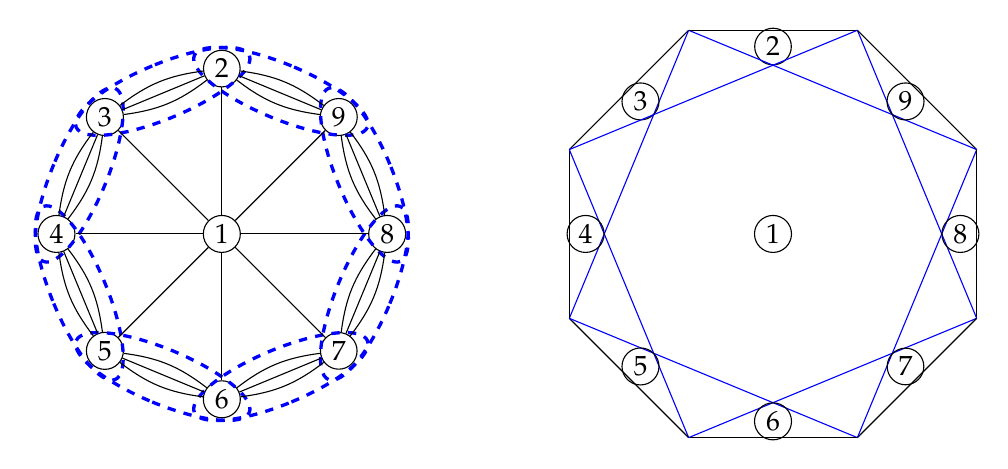
\begin{tikzpicture}[inner sep=1.7pt,scale=.7,pre/.style={<-,shorten <=2pt,>=stealth,thick}, post/.style={->,shorten >=1pt,>=stealth,thick}]
\tikzstyle{every node} = [draw, circle,color=black];
\begin{scope}[shift={(-5,0)}]
\foreach \i in {2,...,9}{
\path (\i*45:3) node  (a_\i) {\i};
}
\foreach \i in {0,...,7}{
\draw [color=blue,dashed,rotate around={22.5+45*\i:(22.5+\i*45:2.8)},line width=1.2] (22.5+\i*45:2.8) ellipse (.5 and 1.7);
}
%\draw [color=blue,dashed,rotate=45,line width=1.2] (45:2.8) ellipse (.7 and 1.7);
\path (0,0) node (c) {1};
\foreach \a/\b in {2/3, 3/4, 4/5, 5/6, 6/7, 7/8, 8/9, 9/2}{
\path (a_\a) edge  (a_\b) edge [bend left=15] (a_\b) edge [bend right=15] (a_\b) edge (c);
}
\end{scope}
\begin{scope}[shift={(5,0)}]
\foreach \i in {2,...,9}{
\draw (22.5+\i*45:4) -- (22.5+45+\i*45:4);
\path (\i*45:3.4) node  (a_\i) {\i};
\draw [color=blue] (22.5+\i*45:4) -- (22.5+90+\i*45:4);
}
\path (0,0) node (c) {1};
\end{scope}
\end{tikzpicture}
\end{center}
\caption[A Family of near Minimum Cuts with an Inside Atom]{%The left graph shows A 7-edge connected graph. The dashed blue lines show a cut class $\C$ of cuts of value at most 8, i.e., (1+1/7)-near minimum cuts. The right image shows the polygon representation of $\C$. The blue lines in the right image are the representing diagonals. This representation has 8 outside atoms and $\{1\}$ is the only inside atom. The system of near minimum cuts corresponding to sets $ (\{2,3\}, \overline{\{2,3\}}), \ldots, (\{8,9\},\overline{\{8,9\}}), (\{9,2\}, \overline{\{9,2\}})$ shows an $8$-cycle for the inside atom $\{1\}$.
Consider the graph on the left and suppose that every edge $e$ has fractional value $x_e =1/7$. This graph then has min cut value 2, with cuts of fractional value at most $2 + 1/7$ circled in blue. Note that this is a connected family $\C$ of near-min cuts, since every adjacent pair of blue cuts cross each other. The right image shows the polygon representation of $\C$. The blue lines in the right image are the representing diagonals. This representation has 8 outside atoms and $\{1\}$ is the only inside atom. The system of near minimum cuts corresponding to sets $ (\{2,3\}, \overline{\{2,3\}}), \ldots, (\{8,9\},\overline{\{8,9\}}), (\{9,2\}, \overline{\{9,2\}})$ shows an $8$-cycle for the inside atom $\{1\}$. See \autoref{def:kcycle}.}
\label{fig:polygonrepresentation}
\end{figure}

\begin{enumerate}
	\item A polygon representation is a convex regular polygon with a collection of \textit{representing diagonals}. All polygon edges and diagonals are drawn using straight lines in the plane. The diagonals partition the polygon into \textit{cells}. 
	\item Each atom of $\C$ is mapped to a cell of the polygon.  If one of these cells is bounded by some portion of the polygon boundary it is {\em non-empty} and we call its atom an \textit{outside atom}. We call the atoms of all other non-empty cells \textit{inside atoms}. Note that some cells may not contain any atom. WLOG label the outside atoms $a_0,\dots,a_{m-1}$ in counterclockwise order, and label the inside atoms arbitrarily. We also label points of the polygon $p_0,\dots,p_{m-1}$ such that outside atom $a_i$ is on the side $(p_i,p_{i+1})$ and $a_0$ is on the side $(p_{m-1},p_0)$. (In future sections we will refer to the special atom called the root, and if it is an outside atom WLOG we will label $a_0$ as the root.)
	\item No cell has more than one incident outer polygon edge.
	\item Each representing diagonal defines a cut such that each side of the cut is given by the union of the atoms on each side. Furthermore, the collection of cuts given by these diagonals is exactly $\mathcal{C}$. 
\end{enumerate}


%We will deal solely with connected components of cuts. In each connected component, we will effectively delete some cuts and then merge others into laminar families. 
The following fact follows immediately from the above discussion:
\begin{fact}
\label{fact:atLeast2Outside}
Any cut $S\in \cC$ (represented by a diagonal of $P$) must have at least two outside atoms.
\end{fact}


\begin{definition}[Outside atoms]
	For a polygon $P$ and a set $S$ of atoms of $P$, we write $O_P(S)$ to denote the set of outside atoms of $P$ in $S$; we drop the subscript when $P$ is clear from context. We also write $O(P)$ (or $O(\cA(\cC))$ where $\cC$ is the connected component of $P$) to denote the set of all outside atoms of $P$.
	
	Note that, given $S \in \cC$, since $S$ may be identified with a set of atoms, $O(S)$ is also well defined. 
\end{definition}



The following observation follows from  the fact that cuts correspond to straight diagonals in the plane and the polygon $P$ is regular:
%\Shayan{We need to justify this observation. Are we using it?}
\begin{observation}[{\cite[Prop 19]{BG08}}] \label{obs:Ocross}
	If $S,S'\in {\cal C}$ cross then $O(S)$ and $O(S')$ cross, and $O(S \cup S') \not= O(P)$.
\end{observation}


\cref{lem:mincutBshowsup} is used in the proof of \cref{lem:extendedprop20}, and depends on the following:

%The following is proved in \cite[Lem 4.1.7]{Ben97}
\begin{theorem}[{\cite[Lem 4.1.7]{Ben97}}]\label{thm:BenCC'}
	Let $\C,\C'$ be two (distinct) connected components of crossing cuts for a family of cuts of $G=(V,E)$. Then, there exists an atom $a\in \cA(\C)$ and $a'\in \cA(\C')$ such that $a\cup a'=V$. 
\end{theorem}


\begin{lemma}\label{lem:mincutBshowsup}
Consider the set of $\eta$-near minimum cuts (NMCs) of $G$ and let $\C$ be a connected component. Let $B\subset\cA(\C)$ be an $\eta$-NMC such that $1<|B|<|\cA(\C)|-1$. Then, $B\in \C$. 
\end{lemma}
\begin{proof}
For the sake of contradiction, suppose $B\notin \C$. Since $B$ is an $\eta$-NMC, it is in some connected component of cuts, say $B\in \C'$, where $\C\ne \C'$. Then, by \cref{thm:BenCC'} there exist atoms $a\in\cA(\C),a'\in\cA(\C')$ such that $a\cup a'=V$.
Observe that by the definition of atoms, each of $a,a'$ is contained in either $B$ or $\overline{B}$. Without loss of generality assume $a\subseteq B$ and $a'\subseteq \overline{B}$. But then, $a\neq B$ since $|B|>1$. So, $a\cup a'\neq V$ which is a contradiction. 
\end{proof}






%\subsubsection{Modified cactus representation}
%
%First we recall the definition of a cactus graph:
%
%\begin{definition}[Cactus Graph]
%\label{def:cactus}
%A {\em cactus graph} is a graph with no cut edges {and} in which no two simple cycles share an edge. \end{definition}
%
%In \cite{Ben97}, it is shown that any collection of cuts admits a modified cactus representation. In particular:
%
%\begin{theorem}[{\cite{Ben97}}]
%\label{thm:tree-representation}
%Let $\cF$  be a collection of cuts of $G=(V,E)$. %, and let $P_i$ be the partition of $V$ corresponding to $\cA(\C)$.
%There exists a cactus $K=(N,E')$ and a mapping $\phi: N \to 2^V$ such that: 
%\begin{enumerate}
%\item $K$ has no cycle of length 3.
%\item There is a 1-to-1 correspondence between the connected components $\cC$ of $\cF$ and the cycles of $K$. In particular, if a connected component $\cC$ and a cycle $L$ are in correspondence, then if $\cC$ has atoms $a_1,\dots,a_k \subseteq 2^V$ (i.e. this forms the coarsest partition of the vertices in $\cC$ as in \cref{def:conn-component-cuts}), $L$ has $k$ vertices and we can order them $v_1,\dots,v_k$ such that $\phi(v_i) = a_i$.
%\item All pairs of atoms $A\in \cA(\C)$ and $B\in \cA(\C')$ with $\C\neq \C'$ that are mapped to a coinciding vertex of the cactus satisfy $\phi(A) \cup \phi(B) = V$.
%\end{enumerate}
%\end{theorem}



%While \cref{sec:poly} does not depend upon any particular random spanning tree distribution, \cref{thm:main} relies heavily on the use of $\lambda$-uniform spanning tree distributions proved in ~\cite{KKO21}.
%For a vector $\lambda:E\to\R_{\geq 0}$, a $\lambda$-uniform distribution $\mu_\lambda$ over spanning trees of $G=(V,E)$ is a distribution where for every spanning tree $T\subseteq E$, $\PP{\mu}{T}=\frac{\prod_{e\in T} \lambda_e}{\sum_{T'} \prod_{e\in T'} \lambda_e}$.
%Now, find a vector $\lambda$ such that for every edge $e\in E$, $\PP{\mu_\lambda}{e\in T}=x_e(1\pm\eps)$, for some $\eps<2^{-n}$. Such a vector $\lambda$ can be found using the multiplicative weight update algorithm \cite{AGMOS10} or by applying interior point methods \cite{SV12} or the ellipsoid method \cite{AGMOS10}. (We note that the multiplicative weight update method can only guarantee $\eps<1/\text{poly}(n)$ in polynomial time.)
%\begin{theorem}[\cite{AGMOS10}]
%\label{thm:maxentropycomp}
%Let $z$ be a point in the spanning tree polytope (see \eqref{eq:spanningtreelp}) of a graph $ G=(V, E)$.
%For any $\eps>0$, a vector $\lambda:E\to\R_{\geq 0}$ can be found such that the corresponding $\lambda$-uniform spanning tree distribution, $\mu_\lambda$, satisfies
%%we define the exponential family distribution
%%$$\tilde{p}(T):=\frac{1}{P}\exp(\sum_{e\in T} \tilde{\gamma}_e)$$ for
%%all $T\in {\cal T}$ where $$P:=\sum_{T\in {\cal T}}\exp(\sum_{e\in T}
%%\tilde{\gamma}_e)$$ then, for every edge $e\in E$,
%$$%\tilde{z}_e :=
%\sum_{T\in {\cal T}: T \ni e} \PP{\mu_\lambda}{T}  \leq (1+\varepsilon)z_e,\hspace{3ex}\forall e\in E,$$
%i.e., the marginals are approximately preserved.  In the above ${\cal T}$ is the set of all spanning trees of $(V,E)$. The running
%time is polynomial in $n=|V|$, $- \log \min_{e\in E} z_e$ and $\log(1/\eps)$.
%\end{theorem}





\subsection{Our polygon notation and the root}\label{sec:polynotation}

All statements in the previous section do not depend on which side of each diagonal we consider. The ambiguity on the sides of the cut considered makes it difficult to define a consistent orientation on the polygon, for example to say whether a cut $A,\overline{A}$ crosses $B,\overline{B}$ ``on the left" or ``on the right." Motivated by this, we identify every cut with the side that does not contain $u_0,v_0$. This has the added benefit of allowing us to apply \cref{lem:treeconditioning} to every cut considered. For every polygon $P$, we call the unique atom $r$ containing $u_0,v_0$ \textit{the root}.  

Recall that, for $\eta>0$, we write $\cN_\eta  \subseteq 2^{V \smallsetminus \{u_0,v_0\}}$ to denote the family of all $\eta$-NMCs of $G_{/e_0}$. %We will always identify each cut  $\delta(S)$ with the side $S$ that does not contain $\{u_0,v_0\}$. 
If $\eta$ is clear in context, we drop the subscript of $\cN_\eta$.
Throughout the paper, we will need to show that various sets $A,B \subseteq V\smallsetminus \{u_0,v_0\}$ cross. Since $u_0, v_0 \in \overline{A \cup B}$ to verify that a pair of sets $A$ and $B$ cross, it suffices to check the three conditions in the following fact.
%By \cref{fact:nou0v0cross} in such cases we only need to verify that $A\cap B,A\smallsetminus B, B\smallsetminus A$ are non-empty (since $A,B$ do not contain $u_0,v_0$). 
\begin{fact}\label{fact:nou0v0cross}
For $A,B\subseteq V\smallsetminus\{u_0,v_0\}$, $A,B$ cross iff
$$A\cap B, A\smallsetminus B, B\smallsetminus A\neq\emptyset.$$	
\end{fact}

As above, unless otherwise specified, we let $\cC$ be a connected component  of cuts in $\cN_\eta$ with corresponding  polygon $P$ for $\eta \leq 1/10$. Again, call the {\em outside} atoms (of $P$) $a_0,\dots,a_{m-1}$, ordered counter-clockwise though these are not necessarily all the atoms in $P$. Note that the root $r$ is not necessarily an outside atom, but if it is, it is the atom labelled $a_0$. 

We use the existence of the root to prove the following two facts. The first fact is a consequence of \cref{obs:Ocross}:

\begin{fact}\label{fact:union-not-everything}
Let $S,S' \in \cC$. Then, $O(S \cup S') \not= O(\cA(\cC))$. 
\end{fact}
\begin{proof}[Proof sketch]
If $S,S'$ are (the non-root) sides of two diagonals of a polygon and there is an atom $r$ which is in neither of them, then there must be a polygon point which is in neither of them. 
%To see this formally, not that if $S,S'$ cross then by \cref{obs:Ocross} we are done. Therefore, we may assume that $A \cap B = \emptyset$, $A \subseteq B$, or $B \subseteq A$. The latter two cases are immediate. So, assume $A \cap B = \emptyset$. 
\end{proof}

The following lemma is the main reason why we can treat each polygon separately in constructing the slack vector mentioned in \cref{sec:overview}. In \cref{sec:twoside}, we are careful to only define positive slack on edges of a polygon that do not have an endpoint in its root.

\begin{fact}\label{fact:edges-internal-to-one-poly}
For any edge $e=\{u,v\}$, there is at most one polygon in which the endpoints of $e$ lie in two different atoms which are not the root of their respective polygons.
\end{fact}
\begin{proof}
	Suppose not, and let $P,P'$ be two polygons in which $u$ and $v$ lie in different atoms that do not contain $r$. By \cref{thm:BenCC'}, there exists an atom $a \in P,a' \in P'$ such that $a \cup a' = V$. Since $u,v$ lie in different atoms (and the atoms of a polygon partition $V$) in both $P,P'$ it must be that (WLOG) $u \in a, v \in a'$. However, since $a \cup a' = V$, $u_0,v_0$ lies in $a$ or $a'$, so either $a$ is the root of $P$ or $a'$ is the root of $P'$, which is a contradiction. 
\end{proof}

%We will call $r$ the root. % such that $a_0$ is the unique atom that contains $e_0=\{u_0,v_0\}$. %We identify each cut in ${\cal C}$ with the side of its representing diagonal that does not contain the root.



We will use {\em``left" synonymously with ``clockwise"} and {\em``right" synonymously with ``counter-clockwise."} 


\begin{definition}[Near min cut notation]
	We will interchangeably refer to a set $S\in\cN_\eta $  by specifying the extreme outside atoms it contains or by specifying the polygon points defining its diagonal. For the former, if $S=(a_l,a_r)$, then  $a_l$ is the leftmost outside atom in $S$ and $a_r$ is the rightmost outside atom in $S$. For the latter, if $S=(p_l,p_r)$, then $p_l$ is the polygon point immediately to the left of $a_l$ and $p_r$ is the polygon point immediately to the right of $a_r$. 
\end{definition}




%For every pair of polygon points $p,q$, consider the two regions defined by the diagonal connecting $p$ to $q$. Let $S=(p,q)$ denote the set of atoms in the region not containing the root. By convention we will write $S=(p_l,p_r)$ such that moving counterclockwise from $p_l$ to $p_r$ we hit all the outside atoms of $S$. For convenience we will also sometimes refer to $S$ as $S=(a_l,a_r)$ where $a_l,a_r$ are outside atoms and $a_l$ is to the left of $a_r$ analogously to above.

%We say an outside atom $a_i$ is \textit{to the left} of another outside atom $a_j$ if $i < j$ and \textit{to the right} otherwise. 

\begin{definition}[$L(p)$, $R(p)$]
For a polygon point $p_i$, let $L(p_i)$  be the largest cut in $\cN_\eta$ containing $a_{i}$ and not $a_{i+1}$ which is crossed on both sides. Let $R(p_i)$ be the largest cut in $\cN_\eta$ containing $a_{i+1}$ and not $a_{i}$ which is crossed on both sides. (Note that $L(p_i),R(p_i)$ do not necessarily exist). See \autoref	{fig:LpRp}.
\end{definition}


 %For example, see \cref{fig:opt-augmentation}. 

%\begin{figure}[htb]
%\begin{center}
%\begin{tikzpicture}[inner sep=1.7pt,scale=.7,pre/.style={<-,shorten <=2pt,>=stealth,thick}, post/.style={->,shorten >=1pt,>=stealth,thick}]
%
%\node at (-3,-2.5) () {$S_L$};
%\node at (3.5,1.5) () {$S_R$};
%
%\node at (1,-3.5) () {$S$};
%
%\tikzstyle{every node} = [draw, circle,color=red];
%\foreach \i in {1,...,8}{
%\path (22.5+\i*45:3) node  (a_\i) {};
%}
%
%\path (a_5) edge [thick, bend right=25, green] (a_4);
%\path (a_5) edge [thick, bend right=15, green] (a_3);
%
%\path (a_7) edge [thick, bend left=25, blue] (a_8);
%\path (a_7) edge [thick, bend left=15, blue] (a_1);
%
%\path (a_7) edge [thick, bend right=15, red] (a_4);
%\path (a_6) edge [thick, bend left=15, red] (a_1);
%\path (a_5) edge [thick, bend right=15, red] (a_2);
%
%\draw [color=black,rotate around={45*4.5:(4.3*45:1.6)},line width=1.2] (4*45:0.8) ellipse (0.9 and 2.7);
%\draw [color=black,rotate around={45*8.5:(1*45:1.6)},line width=1.2] (4.25*45:-2.1) ellipse (0.9 and 2.7);
%
%\draw [color=black,rotate around={45*6.5:(4.3*45:1.6)},line width=1.2] (1.1*45:1.5) ellipse (0.9 and 2.7);
%
%\foreach \a/\b in {1/2, 2/3, 3/4, 4/5, 5/6, 6/7, 7/8, 8/1}{
%\path (a_\a) edge  (a_\b);
%}
%
%\end{tikzpicture}
%\end{center}
%%\caption{$S$ is crossed on the left by $S_L$ and on the right by $S_R$. In green are edges in $\delta(S)^\leftarrow$, in blue edges in $\delta(S)^\rightarrow$, and in red are edges in $\delta(S)^\circ$. }
%\label{fig:crossed-both-sides}
%\end{figure}

The following definitions make formal the notion of ``crossed on one side" and ``crossed on both sides" (introduced in \cref{sec:overview}) for polygons with inside atoms.

\begin{definition}[Left, Right Crossing]
Let $S,S'\in \cC$ such that $S'$ crosses $S$.
For such a pair, we say \textit{$S'$ crosses $S$ on the left} if the leftmost (clockwise-most) outside atom of $O(S' \cup S)$ is in $S'$. %(see \cref{fact:contiguous}).
 Otherwise, we say that \textit{$S'$ crosses $S$ on the right}. Note that by \cref{obs:Ocross}, $O(S),O(S')$ cross. 
%See \cref{fig:polygonexample} for an example.
\end{definition}
\begin{definition}[Crossed on one, both sides]
\label{defn:crossedonetwo}
We say a cut $S$ is \textit{crossed on both sides} if it is crossed by a cut (in $\cC$) on the left and a cut (in $\cC$) on the right and we say $S$ is {\em crossed on one side} if it is crossed only on the left or only on the right. 
\end{definition}

\begin{definition}[$\cN_{\eta,\le 1},\cN_{\eta,1},\cN_{\eta,2}$]
	Let $\cN_{\eta,2} \subseteq \cN_\eta$ be the set of cuts which are crossed on both sides in their respective polygons. Let $\cN_{\eta,1} \subseteq \cN_\eta$ be the set of cuts that are crossed on one side in their respective polygons and finally let $\cN_{\eta,\le 1} = \cN_\eta \smallsetminus \cN_{\eta,2}$ (i.e. the set of cuts which are crossed on one side or not crossed at all).
\end{definition}


Here we give an alternate set-theoretic characterization of $\cN_{\eta,2}$.

\begin{lemma}\label{lem:characterize-N2}
Let $C \in \cN_\eta$. Then, $C \in \cN_{\eta,2}$ if and only if there exist two cuts $A,B \in \cN_\eta$ which cross $C$ such that $(A \smallsetminus C) \cap (B \smallsetminus C) = \emptyset$. 	
\end{lemma}
\begin{proof}
The only if follows from \cref{lem:nointersectionLR}. So, assume there exist two cuts $A,B \in \cN_\eta$ which cross $C$ such that $(A \smallsetminus C) \cap (B \smallsetminus C) = \emptyset$. We will show $C \in \cN_{\eta,2}$. 

Since $A$ and $B$ both cross $C$, it must be that $C,A,B$ are in the same connected component of cuts $\cC \subseteq \cN_\eta$ (i.e. including all cuts in $\cN_{\eta,2}$). Let $P$ be the corresponding polygon.
	
	%By \cref{obs:Ocross}, $O(A)$ and $O(C)$ cross and $O(B)$ and $O(C)$ cross. \anna{Why do you need the last sentence?} 
	Suppose by way of contradiction that $A,B$ both crossed $C$ on the left (if they both cross on the right the argument is similar). Then $A,B$ must both contain the outside atom immediately to the left of the leftmost atom of $C$, which contradicts $(A \smallsetminus C) \cap (B \smallsetminus C) = \emptyset$.
\end{proof}

Consequently, we can give an alternate characterization of $\cN_{\eta,1}$ as the sets which are crossed but are not in $\cN_{\eta,2}$. This will be relevant in \cref{app:oneside}. 

\begin{definition}[$\cC_{2}$]
	For a connected component of cuts $\cC \subseteq \cN_\eta$, let $\cC_{2} = \cC \cap \cN_2$. 
\end{definition}


The following definition is quite important throughout our paper as it is used to specify the set of bad events we use to construct our slack vector (see \cref{sec:overview} for a gentle introduction):

 \begin{definition}[$S_L$, $S_R$]\label{def:SLR}
 For $S \in \cC_2$ let $S_L$ be the near minimum cut crossing $S$ on the left which minimizes $|O(S \cap S_L)|$. If there are multiple sets crossing $S$ on the left with the same minimum intersection, choose the smallest one to be $S_L$. Similarly, let $S_R$ be the near min cut crossing $S$ on the right which minimizes $|O(S \cap S_R)|$, and again choose the smallest set to break ties. See \autoref{fig:S-SR-SL}.
 
 %Equivalently, given $S=(p_l,p_r)$, let $r'$ be the first index in the counterclockwise order starting from $l$ such that there exists a cut $S'$ with rightmost polygon point $p_{r'}$ which crosses $S$ on the left. In such a case, let $S_L$ be the cut minimizing $|O(S_L)|$ among all cuts with rightmost polygon point $p_{r'}$ that cross $S$ on the left. We can define $S_R$ similarly.

% For any set $S$ crossed on both sides such that $S_L, S_R$ cross $S$ on the left and right respectively and minimize their intersections with $S$, 


 \end{definition}
 






%\begin{figure}
%\begin{center}
%\begin{tikzpicture}[inner sep=1.7pt,scale=1,pre/.style={<-,shorten <=2pt,>=stealth,thick}, post/.style={->,shorten >=1pt,>=stealth,thick}]
%\tikzstyle{every node} = [draw,circle,color=black];
%\foreach \i in {0,...,7}{
%\draw (22.5+\i*45:4) -- (22.5+45+\i*45:4);
%\path (90+\i*45:3.4) node  (a_\i) {$a_\i$};
%\draw [color=blue] (22.5+\i*45:4) -- (22.5+90+\i*45:4);
%}
%\path (0,0) node (c) {1};
%\path (90:3.4) node[fill=lightgray]  (a_0) {$a_0$};
%\end{tikzpicture}
%\end{center}
%\caption{In this example, $a_0...a_7$ are the outside atoms, and recall that we identify every diagonal with the side not containing the root. Suppose that $a_0$ is the root (note that the root is not necessarily an outside atom). Then, in this example, $\{a_1,a_2\}$ and $\{a_1...a_6\}$ and are only crossed on the right. $\{a_6,a_7\}$ and $\{a_2...a_7\}$ are only crossed on the left. All other cuts are crossed on both sides. Here we say $a_4$ is to the left of $a_5$ and $a_6$ is to the right of $a_5$. $a_0$ is not comparable to any other atom.}
%\label{fig:polygonexample}
%\end{figure}





\subsection{Properties of inside atoms}

Before proving some new properties of the polygon representation we recall some basic properties of inside atoms from \cite{BG08}:

\begin{definition}[{\cite[Definition 3]{BG08}}]\label{def:kcycle}
A family of sets $C_1,\dots,C_k\subseteq V$, for some $k \ge 3$, forms a $k$-cycle if
\begin{itemize}
\item $C_i$ crosses both $C_{i-1}$ and $C_{i+1}$ (we treat $C_{k+1}$ as $C_1$ and $C_{0}$ as $C_k$);
\item $C_i\cap C_j=\emptyset$ for $j\neq i-1, i$ or $i+1$; and
\item $\bigcup_{1\leq i\leq k} C_i \neq V$.
\item If $k=3$, we have the additional condition $(C_i \cap C_{i+1}) \not\subseteq C_{i-1}$ for $i \in \{1,2,3\}$.
\end{itemize}
\end{definition}


\begin{lemma}[{\cite[Lemma 22]{BG08}}]\label{lem:no-kcycle}
%If  $\eta > \frac{2}{k}$.	
Any $k$-cycle formed by cuts in a connected component ${\cal C}$ of $\eta$-near min cuts satisfies $k\geq 2/\eta$. (Note if $\eta = 0$ then no $k$-cycle exists.)
\end{lemma}

Therefore, for all $2/5$-near min cuts, there are no cycles with length less than 5.
%Generally speaking, since we assume $\eta\ll 1$, the above lemma implies that any $k$-cycle of ${\cal C}$ satisfies $k\gg 3$. 
%This definition gives rise to the formal definition of inside atoms and a related fact:
\begin{lemma}[{\cite[Def 4]{BG08}}]\label{def:inside}
	An atom $a\in \cA(\cC)$ is an inside atom (in the representation defined above) if and only if there is a $k$-cycle $C_1,\dots,C_k\in {\cal C}$, such that $a \cap C_i=\emptyset$ for all $1 \le i \le k$. 
\end{lemma}
See \autoref{fig:polygonrepresentation} for an example of an inside atom and a cycle.

\begin{fact}\label{lem:adjoutsidekcycle}
Let $C_1,\dots,C_k$ be a $k$-cycle for a connected component $\C$ with polygon representation $P$ and $k \ge 5$. For any adjacent pair of outside atoms $a,b\in O(\cA(\cC))$, there is a $1\leq j\le k$ such that $a,b\in C_j$.	
\end{fact}
\begin{proof}
Since $a$ is an outside atom, there is a cut $C_i$ for some $1\leq i\leq k$ such that $a\in C_i$ (otherwise $a$ would be an inside atom). If $b\in C_i$ we are done. Otherwise, $a$ is a rightmost or leftmost outside atom in $C_i$. But then, since $C_i$ is crossed by $C_{i-1}$ and $C_{i+1}$ and $C_{i-1} \cap C_{i+1} = \emptyset$, it follows from \cref{obs:Ocross} (and the fact that both $C_{i-1},C_{i+1}$ contain at least two outside atoms) that either $a,b \in C_{i-1}$ or $a,b \in C_{i+1}$.
%Label the outside atoms of $P$, $o_0,\dots,o_{n-1}$ in clockwise order. WLOG let $C_1,\dots,C_k$ be ordered clockwise such that $O(C_i) = [o_{\ell_i},o_{r_i}]$ such that $\ell_i < r_i$, and $\ell_i < \ell_{i+1} < r_i < r_{i+1} \forall i$ (all mod $n$). 
%WLOG $b$ is the outside atom immediately counterclockwise of $a$. Since $a$ is an outside atom, there is a cut $C_i$ for some $1\leq i\leq k$ such that $a\in C_i$ (otherwise $a$ would be an inside atom). If $b\in C_i$ we are done. 
%Otherwise, $C_i$ is crossed by $C_{i-1}$ and $C_{i+1}$, and say the former crosses $C_i$ such that in the interval $O(C_{i-1} \cup C_i)$, $C_{i-1}$ contains the outside atom furthest counterclockwise. Since $C_{i-1},C_i$ cross, by \cref{obs:Ocross} their outside atoms cross, so $C_{i-1}$ must have both $a,b$.
\end{proof}

\subsection{New properties of polygon representations}
\label{sec:polygonsnewproperties}

The following lemmas build on \cite{Ben95,BG08}. 
\cref{prop20} is a key property of polygons which \cref{lem:extendedprop20} extends: %Some of the statements may have implicitly appeared in those works.


%\begin{lemma}\label{thm:halfplanes}
%Let $ \eta \le  2/5$ and let $P$ be the polygon representation for a connected component $|{\cal C}|$ of at least two $\eta$-NMCs of a (fractionally) 2-edge-connected graph. 
%
%Let $\cH$ be a set of half-planes where each half-plane is one side of a diagonal $D$ of $P$ (corresponding to a represented near min cut) extended to infinity. Suppose that the polytope $\bigcap_{H \in \cH} H$ is non-empty and is entirely contained in the closed set $P$. Let $v_0,\dots,v_{\ell-1}$ be the vertices of $P$ arranged cyclically counterclockwise. Then, perhaps after renaming, it is defined by $\ell$ half-planes $H_0,\dots,H_{\ell-1} \in \cH$ with corresponding diagonals $D_0,\dots,D_{\ell-1}$, where $v_i$ is at the intersection of $D_i$ and $D_{i+1 \pmod{\ell}}$. Note that a segment of each of these diagonals forms a unique edge of the polytope.
%
%%Suppose $H$ is a bounded non-empty intersection of half-planes which lies inside $P$.
% %where each half-plane corresponds to one side of a diagonal $D$ of $P$. If $H$ has $\ell$ vertices, then WLOG it is defined by 
%%If $H$ does not contain any side of $P$ (equivalently, it does not any contain any outside atom) and 
%If $\ell<1/\eta$ then $H$ does not contain any atoms.
%%	The boundary of any non-empty inside cell of the polygon $P$ corresponding to a connected component $\C$ of $\eta$-NMCs   is defined by at least $\Omega(1/\eta)$ diagonals.
%\end{lemma}
%\begin{proof}
%%Define $C_0,\dots,C_{\ell-1} \subseteq V$ such that $C_i$ is all atoms which are not in the halfplane $H_i$. Without loss of generality assume there are no two sets $C_i,C_j$ such that $C_i \subseteq C_j$\footnote{This is because if $C_i \subseteq C_j$ then $H_j \cap P \subseteq H_i \cap P$ which means $H_i$ is redundant in defining $H$.}. 
%%
%%First observe that $H$ is a 2-dimensional polytope and therefore without loss of generality we can assume the diagonals $D_0,\dots,D_{\ell -1}$ are ordered such that the vertices of the polytope $v_0,\dots,v_{\ell-1}$ are arranged cyclically counterclockwise where $v_i$ is the intersection of $D_i$ and $D_{i+1}$ 
%For the rest of the proof take all indices mod $\ell$. We will call a vertex $v_i$ \textit{external} if $D_{i}$ and $D_{i+1}$ intersect at a vertex of $P$ and \textit{internal} otherwise.
%
%We prove the claim by induction over $r$ that if $H$ has $r$ external vertices and $\ell+r < 2/\eta$, then $H$ contains no atoms. This will suffice to prove the theorem because assuming $\ell < 1/\eta$, we have $\ell+r<2/\eta$ (using that $r\leq \ell$).
%
%First assume $r=0$. Then, $C_{i}$ crosses $C_{i+1}$ for all $i$. By way of contradiction suppose $H$ contains an (inside) atom $a$. We claim that for every $i,j$ where $j \not\in \{i-1,i,i+1\}$, we have $C_i \cap C_j = \emptyset$. Suppose not. Then since $C_i \not\subseteq C_j$,  $C_j \not\subseteq C_i$, $a \not\in C_i,C_j$, it follows that $C_i,C_j$ cross and therefore the diagonals $D_i,D_j$ intersect in the interior of $P$, which is a contradiction.%. Now $D_0,\dots,D_i,D_j,\dots,D_{\ell-1}$ contains $H$ and has no external vertices and thus contradicts the minimality of $H_0,\dots,H_{\ell-1}$.  
%
%Therefore by minimality, $C_i \cap C_j = \emptyset$ if $j \not= i-1,i$ or $i+1$. So, $C_0,\dots,C_{\ell-1}$ is a $k$-cycle for $a$: since there are no external vertices, $C_i$ crosses $C_{i+1}$ for all $i$, and $\bigcup_{i=0}^{\ell-1} C_i \not= V$ since $a \not\in C_i$ for all $i$. But by \cref{lem:no-kcycle}, $\ell \ge 2/\eta$, which is a contradiction.
%
%Now, suppose the claim is true when the number of external vertices is at most $r$; we will prove it holds when the number is $r+1$.  
%
%Again, by way of contradiction suppose there is an inside atom $a$ in $H$. Then there is a $k$-cycle for $a$ in $\cC$,  say $L_1,\dots,L_k$. Now pick an arbitrary external vertex $v_i$ of $H$. Let $o_l,o_r \in O(\cA(\cC))$ be the adjacent outside atoms immediately clockwise and counterclockwise of $v_i$. Therefore, since $k \ge 4$, by \cref{lem:adjoutsidekcycle}, there exists some $j$ such that $o_l,o_r \in L_j$. Let $H_{\ell}$ be the halfspace corresponding to the side of $L_j$ containing $a$. Now consider the set of halfspaces $H_0,\dots,H_{\ell-1},H_{\ell}$. Note that $H'=\bigcap_{i=0}^{\ell} H_i \subsetneq H$ because $v_i \not\in H_\ell$. Therefore, $H'$ has at least one fewer external vertex and no sides of the polygon. Since $\ell+1+(r-1) \le 2/\eta$, by the induction hypothesis, $H'$ has no inside atoms which is a contradiction with the existence of $a$. 
%\end{proof}

%\begin{lemma}[{\cite[Lemma 12]{BG08}}]\label{lem:kcycle}
%	Let $S \in {\cal C}$ and $f \in S$ be an inside atom. Let $C_1...C_k$ be a cycle for $f$. Then there exists an $i$ such that $C_i \subset S$. 
%\end{lemma}


\begin{proposition}[{\cite[Proposition 20]{BG08}}]\label{prop20}
For any connected component ${\cal C}$ of $\eta$-near min cuts with $\eta \leq 2/5$ with polygon representation $P$, and any $S_1, S_2 \in \mathcal{C}$ with $S_1 \not= S_2$ we have $O_P(S_1) \neq O_P(S_2)$.
\end{proposition}
%\anna{The polygon representation is unique, right? Also, are atoms $\eta$ near mincuts?}

\begin{lemma}\label{lem:extendedprop20}
Let $P$ be the polygon representation  for a connected component $|{\cal C}|>1$ of $\eta$-NMCs of a (fractionally) 2-edge connected graph $G$ with atom set $\cA(\cC)$. If $A,B\subsetneq \cA(\cC)$ are two  $2/5$-NMCs with $O_P(A) = O_P(B)\ne \emptyset$ and there is an atom $r\in \cA(\C)$ such that $r\notin A,B$, then $A=B$ \footnote{As indicated earlier, $r$ is called the root of the polygon $P$}.
%Let $P$ be a polygon representation of a connected component ${\cal C}$ of $2+\eta$ near minimum cuts for some $\eta\le 2/5$. For any $A,B\subseteq \cA(\cC)$  such that $A\neq B$ and $O(A) = O(B)\neq\emptyset$   we have $\max\{x(\delta(A)), x(\delta(B))\} \geq 12/5$.
\end{lemma}
\begin{proof}
%Let $\cC$ be a connected component of $\eta$-NMCs of a $k$-edge connected graph $G$. 
Take the graph $G$ and contract each atom of $\cA(\cC)$ to a single node. Call the resulting graph $G'$.
Clearly, $G'$ is still $2$-edge connected  since $G$ is $2$-edge-connected and all cuts in $\cC$ are represented in $G'$.
Now, consider the set of non-singleton $2/5$-near-min-cuts of $G'$. This set has a unique connected component of crossing cuts because any new (non-singleton) cut $S\notin \cC$ is crossed by a cut in $\cC$. (Suppose not: then, no cut on the atoms of $S$ crosses a cut on the atoms of $\overline{S}$, which contradicts that $\cC$ forms a connected component.) Call this component of cuts $\cC'$ and the corresponding polygon $P'$. It follows that $\cA(\cC)=\cA(\cC')$ (more precisely, a set  $S \subseteq V$ is an atom in $\cA(\cC)$ if and only if it is an atom in $\cA(\cC')$): no two atoms  from $P$ can be merged in $P'$ because we have not deleted any cuts, and no atoms in $P$ can be split in $P'$ because we have contracted them.
 While some outside atoms of $P$ may become inside atoms in $P'$, it follows by \cref{def:inside} that any inside atom of $P$ remains an inside atom in $P'$ (as any $k$-cycle of $\cC$ is also a $k$-cycle of $\cC'$). Therefore, 
 $$O_{P'}(A) = O_{P'}(B).$$
 
 Therefore, if $A,B \in \cC'$, by \cref{prop20}, $A=B$. So it remains to show that $A,B \in \cC'$. First, assume $2 \le |A| \le |\cA(\cC')|-2$ and $2 \le |B| \le |\cA(\cC')|-2$. Then, by \cref{lem:mincutBshowsup}, $A,B\in\cC'$ and we are done.
   
%Therefore we can look at its polygon representation for cuts with $x(\delta(S)) \le 2+2\eta$ and it will have the same set of atoms as $P$: no two atoms can be merged because we have not deleted any cuts (the atoms were already minimal in $P$), and no atoms can be split because we have contracted them in $G'$. 

%However, the polygon may change; let $P'$ be the resulting polygon with connected component ${\cal C}'$. 
 %and set $$\eta'=\max\{x(\delta(A)), x(\delta(B))\}-2.$$
Now, we claim that $2 \le |A| \le |\cA(\cC')|-2$ and $2 \le |B| \le |\cA(\cC')|-2$, which by the above would complete the proof. For contradiction, assume $A\neq B$ and $|A|=1$ or $|A|=|\cA(\cC')|-1$. First assume $|A|=1$. Since $B\neq A$, $O_{P}(A)=O_P(B)\neq\emptyset$, and every polygon has at least three outside atoms, $2 \le |B| \le \cA(\cC) - 2$. By \cref{lem:mincutBshowsup}, $B\in \cC'$. Yet this implies that $B$ has at least two outside atoms in $P'$ (and therefore in $P$), which contradicts $O_{P'}(A) = O_{P'}(B)$. Otherwise, $|A| = |\cA(\cC')|-1$. Using that $A \not= B$ and $r \not\in A,B$, it follows that $B$ has at most $|\cA(\cC')|-2$ atoms. Again using that every polygon has at least three outside atoms, this implies $|B| \ge 2$. So similarly to above, we have $B \in \cC'$. Therefore, $|O_{P'}(B)| \le |O(P')|-2$ which contradicts that $|A|=|\cA(\cC')|-1$ using $O_{P'}(A)=O_{P'}(B)$.
%$B$ is neither a singleton nor a complement of a singleton; in the latter case $B$ must have at least two outside atoms (because every polygon has at least three outside atoms) which is a contradiction to $A$ being a singleton. 
% So, by \cref{lem:mincutBshowsup} $B\in \cC'$. 
%And, by definition of the polygon $P'$, $B$ must have at least two outside atoms in $P'$.  Since any outside atom of $P'$ is an outside atom of $P$, $|O_P(A)|=|O_P(B)| \ge 2$ which is a contradiction with $A$ being a singleton.
%Otherwise, assume $A$ is a complement of a singleton. By similar analogy $B$ is not a singleton. If $B$ is also a complement of a singleton, then we must have $A=B$ since $r\neq A,B$ and we are done. Otherwise, by \cref{lem:mincutBshowsup} $B\in \cC'$. So, $2\leq O_{P'}(\overline{B}) \leq O_P(\overline{B})=O_P(\overline{A})$ but that is a contradiction with $A$ being a complement of a singleton.
%However, since $O_P(A)\neq \emptyset$, we must have $|O_P(A)|=|O_P(B)|\geq 2$, which is a contradiction. %we must have $O_{P'}(A)\neq O_{P'}(B)$ which is a contradiction.
\end{proof}



%\begin{lemma}[\anna{Alternative version}]\label{lem:extendedprop20-alt}
%Let $ \eta \le  \eta' \le  2/5$
%	and let $P$ be the polygon representation  for a connected component ${\cal C}$ of $\eta$-NMCs with atom set $\cA(\cC)$. If $A,B\subseteq \cA(\cC)$ are two  $\eta'$-NMCs with $O_P(A) = O_P(B)\ne \emptyset$, then $A=B$.
%\end{lemma}
%\begin{proof}
%Consider the graph $G'$ arising from contracting all sets of vertices in $G$ corresponding to atoms of $\cA(\cC)$. This is still a (fractionally) 2-edge-connected graph since $G$ is 2-edge-connected. 
%Let $\cC'$ be the set of  $\eta'$-NMCs of $G'$. Since $\cC\subseteq \cC'$, it is a connected component and therefore has a polygon representation $P'$ with $\cA(\cC) = \cA(\cC' )$ (no two atoms  from $P$ can be merged in $P'$ because we have not deleted any cuts, and no atoms in $P$ can be split in $P'$ because we have contracted them.) Moreover, by \cref{def:inside}, every inside atom of $P$ is still an inside atom of $P'$ since it has a corresponding $k$-cycle. 
%
%In addition, since $A$ and $B$  are both cuts in $\cC'$, each is represented by a diagonal, and therefore, by \cref{fact:atLeast2Outside}, $|O_{P'}(A)|, |O_{P'}(B)| \ge 2$.
%
%Finally, if $D$ is the subset of outside atoms in $O_P(A)$ that become inside atoms in $P'$, then, since $O_{P}(A) =  O_{P}(B)$, we have 
%$O_{P'}(A)  = O_{P}(A)\smallsetminus D = 
%O_{P'}(B)$. 
%It follows by \cref{prop20} that, since $A$ and $B$ have the same outside atoms in $P'$, they are the same set. 
%\end{proof}

%\begin{corollary}
%Let $S$ be any subset of outside atoms in $\cA(\cC)$ and let $S'$ be a collection of internal cells such that $S \cup S'$ is an $\eta' \le 2/5$ NMC. Then $S'$ contains no atoms.
%\end{corollary}

We generalize \cref{obs:Ocross} in the next lemma.
\begin{lemma}\label{lem:OABcross}
	Let $P$ be a polygon representation of a connected component ${\cal C}$ of $\eta$ NMCs of a (fractionally) 2-edge-connected graph $G$ for some $\eta \leq 2/5$. For any $2/5$ NMCs $A,B\subseteq \cA(\cC)$ with $O(A),O(B)\neq \emptyset$, if $A,B$ cross, then $O(A), O(B)$ cross and $O(A \cup B) \not= O(\cA(\cC))$.
\end{lemma}
\begin{proof}
Similar to the previous lemma, consider the graph $G'$ arising from contracting all atoms of $\cA(\cC)$ and let $\cC'$ be the (unique) connected component of non-singleton $2/5$-near-min-cuts of $G'$ with corresponding polygon $P'$. 
As before, $\cA(\cC')=\cA(\cC)$ and $O(\cA(\cC')) \subseteq O(\cA(\cC))$.
%and the outside atoms of $\cC'$ are a subset of the outside atoms of $\cC$.

Notice that since $A,B$ cross (in $P$), each of them contains at least two atoms of $P$.
Therefore, since $A,B$ are $2/5$ NMCs and $A,B$ are not singletons, we must have $A,B\in \cC'$.  
Since $A,B$ cross in $P$ and $\cA(\cC')=\cA(\cC)$, they also cross in $P'$. By \cref{obs:Ocross}, it follows that $O_{P'}(A)$ and $O_{P'}(B)$ cross. Recall that outside atoms of $\cA(\cC)$ may become inside atoms of $\cA(\cC')$, but inside atoms of $\cA(\cC)$ remain inside atoms in $\cA(\cC')$. So, $O_P(A)$ and $O_P(B)$ cross as well (in particular it also follows that $O(A \cup B) \not= O(\cA(\cC))$).
\end{proof}


\subsubsection{Almost diagonal cuts and the chain lemma}

In some cases, we will need to refer to cuts which are generated by intersections of diagonals in $\cC$. Such cuts are a subset of the following class:

\begin{definition}[Almost Diagonal Cuts]
Let $\cC$ be a connected component of cuts in $\cN_\eta$. We say a set of atoms $S \subseteq \cA(\cC)\smallsetminus \{r\}$ is an {\em almost diagonal cut} if:
\begin{enumerate}
\item $S$ is a $2\eta$-near min cut,
\item $\emptyset \neq O(S) \subsetneq O(\cA(\cC))$,
\item $O(S)$ forms a contiguous interval in the polygon.
\end{enumerate}
Notice that by definition any cut in $\cC$ is  an almost diagonal cut. 
%We also reserve the term $\epsilon$-almost diagonal cut to signify the above definition for cuts $S$ which are $\epsilon$ near min cuts.
\end{definition}

When we reference almost diagonal cuts in the rest of the paper, we will always assume $\eta \le 1/5$. Notice that given any two $A,B \in \cN_\eta$, $A \cap B, A \smallsetminus B, B \smallsetminus A$ are almost diagonal cuts.

The following fact implies that one can naturally define left/right crossing analogous to \cref{def:SLR} for almost diagonal cuts. The following is a consequence of \cref{lem:OABcross}:
\begin{fact}\label{fact:contiguous}
Let $A,B$ be two crossing almost diagonal cuts. Then, $O(A)$ and $O(B)$ cross. In addition, neither $O(A \cup B)$ nor $O(A \cap B)$ contain all outside atoms and each of $O(A \cup B)$ and $O(A \cap B)$ form a contiguous interval of  outside atoms.
\end{fact} 
%This is because if $O(A \cap B)$ is not a contiguous interval, then it must be that $O(A \cap B) = O(\cA(\cC))$. \anna{Proof by picture?} Similarly, by \cref{lem:OABcross}, if two almost diagonal cuts cross, their outside atoms cross as well. 

\begin{lemma}\label{lem:nointersectionLR}
For an almost diagonal cut $S$ with leftmost atom $a_l$ and rightmost atom $a_r$, let $L \in \cC$ cross $S$ on the left and $R \in \cC$ cross $S$ on the right. Then, if $\eta \le 1/5$, $(L \smallsetminus S) \cap (R \smallsetminus S) = \emptyset$. 	
\end{lemma}
\begin{proof}
	Suppose $(L \smallsetminus S) \cap (R \smallsetminus S) \not= \emptyset$. We will show that $L,R,S$ form a 3-cycle (\cref{def:kcycle}) which cannot exist. To show this (using that the root atom $r \not\in S \cup L \cup R$), it is enough to prove that all pairs cross and none of the three sets is a superset of the intersection of the two others. First, by assumption $L$ and $R$ cross $S$. $L$ and $R$ cross because $a_r \in R \smallsetminus L, a_l \in L \smallsetminus R$, so neither is a subset of the other, and because we assumed $(L \smallsetminus S) \cap (R \smallsetminus S) \not= \emptyset$ their intersection is nonempty. 
	
	In addition, we have $S \cap L \not\subseteq R$ because $a_l \in S \cap L$ but not in $R$. Similarly $S \cap R \not\subseteq L$. Finally, $L \cap R \not\subseteq S$ by the assumption $(L \smallsetminus S) \cap (R \smallsetminus S) \not= \emptyset$. Therefore $S,L,R$ form a 3-cycle which is a contradiction as $S,L,R$ are all $2/5$-near min cuts.
\end{proof}

A fundamental property of the cactus representation is that  the set of min cuts $A_1,\dots,A_k$ crossing a min cut $S$ form two laminar families inside $S$. In other words, perhaps after renaming we may assume $A_1 \cap S \subseteq A_2 \cap S \dots \subseteq A_j \cap S$ and $A_{j+1} \cap S \subseteq \dots \subseteq A_k \cap S$.

It is not immediately obvious that such a property extends to polygons because of the existence of inside atoms. Nonetheless, the following lemma demonstrates that this property is also true of near min cuts provided that $\eta$ is small enough. It is an immediate corollary of \cref{lem:crosschain}. 
\begin{lemma}[Chain Lemma]\label{lem:crosschain} 
%\label{cor:ChainRule}
Let  $S$ be an almost diagonal cut where $O(S)$ contains all outside atoms from $a$ to $b$. In addition, let $A_1,\dots,A_k\in\cC$ be the collection of $\eta$-near-min cuts crossing $S$ on the left. Then there is a permutation, $\pi:[k]\to [k]$ such that 
$$S\cap S_L=S\cap A_{\pi(1)} \subseteq \dots  \subseteq S\cap A_{\pi(k)}$$ 
i.e., their intersections with $S$ form a chain. The same statements also hold for cuts crossing $S$ on the right.	
\end{lemma}

\begin{lemma}\label{lem:crosschain}
Let $S$ be a near diagonal cut with leftmost outside atom $a$ and rightmost outside atom $b$. Furthermore, let $A=[a_1,a_2],B=[b_1,b_2]\in \cC$ be cuts which cross $S$ on the right. If $\eta \leq 1/10$ and in the interval of the outside atoms of $O(S)$, $a_1$ is to the left of $b_1$, then $B \cap S \subseteq A \cap S$. 
In the special case that $a_1=b_1$, we have $S\cap A=S\cap B$.  
\end{lemma}
\begin{proof}
First assume $b_1\neq a_1$. Since $b_1$ is to the right of $a_1$, and $A,B$ cross $S$ on the right, $O(A\cap S\cap B)=O(S\cap B)\neq\emptyset$ (as both sets have all outside atoms between $b_1$ and $b$). Note that $B$ crosses $A \cap S$. This is because $B$ has an atom outside of $S$ (as it crosses $S$ itself), $a_1 \in A \cap S \smallsetminus B$, and $b_1 \in A \cap S \cap B$. So by \cref{lem:cutdecrement} $A \cap S \cap B$ is a $4\eta$ near min cut. In addition, $S \cap B$ is a $3\eta$ near min cut since $B$ crosses $S$. Therefore, since $4\eta\leq 2/5$, by \cref{lem:extendedprop20} $A\cap S\cap B=S\cap B$.
%applied to the sets $A\cap S\cap B$ and $S\cap B$, either $A\cap S\cap B = S\cap B$ or $\max\{x(\delta(A\cap S\cap B)), x(\delta(S\cap B))\}\geq 12/5$. The latter contradicts $\eta \leq 1/10$, so we must have the former which implies $S\cap B\subseteq S\cap A$.

In the special case that $a_1=b_1$, $O(A\cap S)=O(B\cap S)\neq\emptyset$ has all outside atoms between $a_1=b_1$ and $b$.
Since $A\cap S,B\cap S$ are $3\eta$ near min-cuts, by \cref{lem:extendedprop20}, we must have $A\cap S=B\cap S$ as desired.
%can simply run the above argument with role of $A,B$ swapped; and that would imply $S\cap B=S\cap A$.
 %However $O(A_1 \cap A_2 \cap S) = [a_2 \dots b]$ and $O(A_2 \cap S) = [a_2 \dots b]$, so $O(A_1 \cap A_2 \cap S) = O(A_2 \cap S)$.  However this implies $A_2 \cap S \subseteq A_1 \cap S$, proving the lemma.
	%First note $A_1 \cap A_2 \cap S \not= \varnothing$ since $A_1,A_2$ must contain the atom $b$.  By our assumption there exists an atom $f \in (A_2 \cap S) \smallsetminus A_1$, and it must be an inside atom since $O(A_2 \cap S) \subseteq O(A_1 \cap S)$ as $a_1$ is to the left of $a_2$. 
\end{proof}

\subsection{Another structural property of inside atoms}

The following lemma is not explicitly used in the proof of the main theorem, but the statement may be useful to guide the reader's intuition (or in other settings where near min cuts arise). For example, it implies that the yellow region is empty in \cref{fig:ErL=ErS}.

\begin{lemma}\label{thm:halfplanes}
Let $ \eta \le  2/5$ and let $P$ be the polygon representation for a connected component $|{\cal C}|>1$ of $\eta$-NMCs of a (fractionally) 2-edge-connected graph. Suppose $H$ is the intersection of half-planes\footnote{Technically, half-polygons.} $H_0,\dots,H_{\ell-1}$ corresponding to diagonals $D_0,\dots,D_{\ell-1}$ of $P$ that has a positive area. If $H$ does not contain any side of $P$ (equivalently, it does not any contain any outside atom) and $\ell<1/\eta$ then $H$ does not have any inside atoms.
%	The boundary of any non-empty inside cell of the polygon $P$ corresponding to a connected component $\C$ of $\eta$-NMCs   is defined by at least $\Omega(1/\eta)$ diagonals.
\end{lemma}
\begin{proof}
Define $C_0,\dots,C_{\ell-1} \subseteq V$ such that $C_i = \cA(\C) \cap \overline{H_i}$, i.e. all atoms which are not in the halfplane $H_i$. Without loss of generality assume there are no two sets $C_i,C_j$ such that $C_i \subseteq C_j$\footnote{This is because if $C_i \subseteq C_j$ then $H_j \cap P \subseteq H_i \cap P$ which means $H_i$ is redundant in defining $H$.}. 

First observe that $H$ is a 2-dimensional polytope and therefore without loss of generality we can assume each $D_i$ defines a side of $H$ and $D_0,\dots,D_{\ell -1}$ are ordered such that the vertices of the polytope $v_0,\dots,v_{\ell-1}$ are arranged cyclically counterclockwise where $v_i$ is the intersection of $D_i$ and $D_{i+1}$ (where for the rest of the proof we take all indices mod $\ell$). We will call a vertex \textit{external} if it is a polygon point of $P$ and \textit{internal} otherwise. 

We prove the claim by induction over $r$ that if $H$ has $r$ external vertices and $\ell+r < 2/\eta$, then $H$ is empty. Note that if $\ell < 1/\eta$, since $r\leq \ell$, we have $\ell+r<2/\eta$ which proves the theorem.

First assume $r=0$. Then, $C_{i}$ crosses $C_{i+1}$ for all $i$. By way of contradiction suppose $H$ contains an (inside) atom $a$. Without loss of generality, assume that $H_0,\dots,H_{k-1} \subseteq H_0,\dots,H_{\ell-1}$ (perhaps after renaming) is the minimal set of half-planes that contain $H$ and have no external vertices. We claim that there are no indices $i,j$ and $j \not= i-1,i,$ or $i+1$ such that $C_i \cap C_j \not= \emptyset$. Since $C_i \not\subseteq C_j$,  $C_j \not\subseteq C_i$, $a \not\in C_i,C_j$, it follows that $C_i,C_j$ cross and therefore the diagonals $D_i,D_j$ intersect in the interior of $P$. Now $D_0,\dots,D_i,D_j,\dots,D_{k-1}$ contains $H$ and has no external vertices and thus contradicts the minimality of $H_0,\dots,H_{k-1}$.  

Therefore by minimality, $C_i \cap C_j = \emptyset$ if $j \not= i-1,i$ or $i+1$. So, $C_0,\dots,C_{k-1}$ is a $k$-cycle for $a$: since there are no external vertices, $C_i$ crosses $C_{i+1}$ for all $i$, and $\bigcup_{i=0}^{\ell-1} C_i \not= V$ since $a \not\in C_i$ for all $i$. By \cref{lem:no-kcycle}, $k \ge  2/\eta$, which is a contradiction, because $k \le \ell < 1/\eta$. 

Now, suppose the claim is true when the number of external vertices is at most $r$; we will prove it holds when the number is $r+1$.  

Again, by way of contradiction suppose there is an inside atom $a$ in $H$. Then there is a $k$-cycle for $a$, $L_1,\dots,L_k \in \cC$. Now pick an arbitrary external vertex $v_i=p_j$ of $H$ for some $j$. Let $a_{j-1},a_{j} \in O(\cA(\cC))$ be the adjacent outside atoms immediately to the clockwise and counterclockwise of $p_j$. Therefore, by \cref{lem:adjoutsidekcycle}, there exists some $j$ such that $a_{j-1},a_j \in L_j$. Let $H_{\ell}$ be the halfspace corresponding to the side of $L_j$ containing $a$. Now consider the set of halfspaces $H_0,\dots,H_{\ell-1},H_{\ell}$. Note that $H'=\bigcap_{i=0}^{\ell} H_i \subsetneq H$ because $v_i=p_j \not\in H_\ell$. Therefore, $H'$ has at least one fewer external vertex and no sides of the polygon. Since $\ell+1+(r-1) \le 2/\eta$, by the induction hypothesis, $H'$ has no inside atoms which is a contradiction with the existence of $a$. 
\end{proof}



%\begin{lemma}[\anna{Alternative version of the chain rule}]
%Let $S$ be an almost diagonal cut with respect to polygon $P$ of $\eta$-NMCs,  and suppose that  $A$ and $B$ are cuts in $\cC$ that both cross $S$ on the left (or on the right).
%Then $A\cap S \subseteq B \cap S$ (or $B\cap S \subseteq A \cap S$). \end{lemma}
%
%\begin{proof}
%By \cref{lem:cutdecrement}, $S \cap A$ and $S \cap B$ and $S \cap A \cap B$ are all $4\eta$ NMCs.
%Therefore, by \cref{lem:extendedprop20-alt}, if $O(S \cap A) = O(S \cap B)$, then $S \cap A=S \cap B$ and we are done. Otherwise, since $A$ and $B$ both cross $S$ on the left, we can assume wlog that $O(S \cap A) \subsetneq O(S \cap B)$.  But since $S\cap A$ and $S \cap A \cap B$ contain the exact same set of outside atoms ($O(S \cap A)$),  by \cref{lem:extendedprop20}  they must be the same set. This implies that $I(S \cap A \cap B)= I(S\cap A)$ and therefore, $I(S\cap A) \subseteq I (S \cap B)$, completing the proof.
%\end{proof}










\section{Proof of the main theorem}\label{sec:twoside}

\subsection{Notation and a preliminary lemma}

We will use the same set of definitions for bad events and increase sets that we did in \cref{sec:overview} for polygons without inside atoms. For the benefit of the reader we repeat them here. Recalling the definitions from \cref{sec:polynotation}, partition each set $\delta(S)$ into three sets $E^\leftarrow(S), E^\rightarrow(S)$ and $E^\circ(S)$ such that
 \begin{align*}
 	E^\leftarrow(S) &= E(S \cap S_L, S_L \smallsetminus S) \\
 	 E^\rightarrow(S) &= E(S \cap S_R, S_R \smallsetminus S) \\
 	 E^\circ(S) &= \delta(S) \smallsetminus (E^\leftarrow(S) \cup E^\rightarrow(S))
 \end{align*}
In addition we define the left and right bad events:
\begin{align}
	B^\rightarrow (p) &= \mathbb{1}\{|E^{\rightarrow} (L(p)) \cap T|\ne 1\text{ or }|E^\circ (L(p)) \cap T|\ne 0\}\notag\\
B^\leftarrow (p) &= \mathbb{1}\{|E^{\leftarrow} (R(p)) \cap T|\ne 1\text{ or }|E^\circ (R(p)) \cap T|\ne 0\}. \label{defn:badevents2}
\end{align}
If $L(p)$ does not exist, simply assume the left bad event never occurs, and similarly if $R(p)$ does not exist assume the right bad event never occurs.

Define $L(p)^{\cap R} := L(p) \cap L(p)_R$, and let $L^*(p) \in \cC$ be the cut crossing $L(p)^{\cap R}$ on the left that {\em maximizes}  $|O(L^*(p) \cap L(p)^{\cap R})|$ (and similarly $R^*(p)$ to maximize the intersection with $O(R(p)^{\cap L})$ on the right). If $L^*(p)$ does not exist, i.e. no cut crosses $L(p)^{\cap R}$ on the left, set $L^*(p) = \emptyset$, and similarly for $R^*(p)$. We let:

\begin{figure}[htb]\centering
	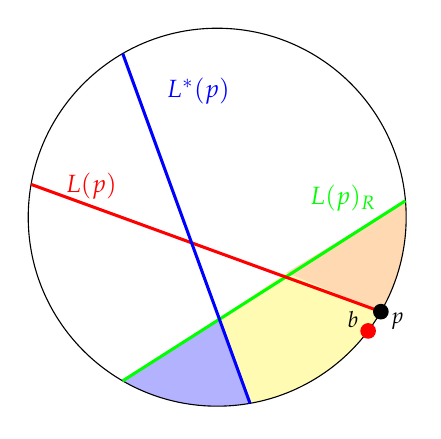
\begin{tikzpicture}[scale=0.8]
		\fill [color=blue!30] (240:3) -- (0.03,-1.61) -- (280:3)  arc (280:240:3); 
		\fill [color=yellow!30] (280:3) -- (0.03,-1.61) -- (1.1,-0.88) -- (330:3) arc (330:280:3);
		\fill [color=orange!30] (330:3) -- (1.1,-0.88) -- (5:3) arc (365:330:3);
		\draw (0,0) circle (3);
		\draw [color=green,line width=1.1pt] (240:3) -- (5:3);
		\node [color=green] at (2,0.3) () {\small $L(p)_R$};
		\draw [color=red, line width=1.1pt] (170:3) --   (330:3);
		\node [color=red] at (-2,0.5) () {\small $L(p)$};
		\draw [color=blue,line width=1.1pt] (120:3) -- (280:3);
		\node [color=blue] at (-0.3,2) {\small $L^*(p)$};
		\node [color=black,circle,fill=black,inner sep=2] at (330:3) () {};
		\node at (330:3.3) () {\footnotesize$p$};
		\node [circle,fill=red,inner sep=2] at (323:3) {};
		\node at (323:2.7) () {\footnotesize $b$};
	\end{tikzpicture}
	\caption{\small Recap of some basic definitions: $L(p)$ is the cut crossed on both sides with rightmost polygon point $p$ (and contains all atoms below the red diagonal. $L(p)_R$ is the cut crossing $L(p)$ on the right that minimizes the number of outside atoms in $L(p)^{\cap R} = L(p) \cap L(p)_R$, i.e., in yellow + blue.	Note that the cut $L(p)^{\cap R}$ contains all atoms in the yellow and blue regions (which may include inside atoms).  Since this region is the set difference of two $\eta$ near min cuts, it is a $2\eta$ near min cut. $L^*(p)$ is the cut crossing $L(p)^{\cap R}$ on the left that maximizes the number of outside atoms in the intersection, i.e., maximizes the number of outside atoms in the blue region. $E^\rightarrow (L(p))$ are the edges between atoms in the yellow region and atoms in the orange region. There is one edge in the tree that is in $E^\rightarrow (L(p))$ with probability $1-O(\eta)$ and when this event does not occur, $B^\rightarrow(p)$ occurs. ($B^\rightarrow(p)$ also occurs if $|E^\circ (L(p)) \cap T|\ne 0$.)}
\end{figure}

\begin{align}
	E(B^\rightarrow (p)) &:= E( L(p)^{\cap R} \smallsetminus L^*(p), L(p)_R \smallsetminus  L(p)^{\cap R})  \notag\\
	E(B^\leftarrow (p)) &:= E( R(p)^{\cap L} \smallsetminus R^*(p), R(p)_L \smallsetminus  R(p)^{\cap L})\label{defn:slackincrease2}.
\end{align}

The following important lemma is the generalization of \cref{claim:1} from \cref{sec:overview} to the case in which there may be inside atoms. It uses that by \cref{lem:extendedprop20} many regions of the polygon do not contain inside atoms.

%\Nathan{Check this next proof for clarity}

\begin{lemma}\label{lem:samerightEPsameedgeset}
	Let $A, B \in \cC_{2}$ such that $A=(a_1,a_r)$ and $B=(a_2,a_r)$ share a rightmost polygon point $p_r$. Then, $A_R = B_R$ and $E^\rightarrow(A) = E^\rightarrow(B)$.
\end{lemma}
\begin{proof}
	WLOG assume $A \subseteq B$. First, we will prove that if a cut $R$ crosses $A$ on the right, it also crosses $B$ on the right. So, let $R$ be a set crossing $A$ on the right. Then, since $R$ contains $a_{r}$, $R \cap B \not= \emptyset$. Furthermore, $R$ contains atom $a_{r+1}$, so $R \not\subseteq B$. Finally, $B$ contains $a_1$ since $A \subseteq B$ yet $R$ does not. Therefore, $R$ crosses $B$ on the right. 
	
	Therefore, by \cref{def:SLR} $A_R = B_R$ since the set of cuts crossing $B$ on the right is a superset of cuts crossing $A$ on the right and any cut which crosses $B$ but not $A$ contains all atoms of $A$, so would have a larger intersection with $O(B)$. (If two sets have the same intersection with $O(A)$ we use the same tie-breaking rule for both $A_R$ and $B_R$.)   
	
	Now we prove that $E^\rightarrow(A) = E^\rightarrow(B)$. Let $R=A_R=B_R$. It suffices to show that $R \cap A = R \cap B$ and $R \smallsetminus A = R \smallsetminus B$ because any edge $e \in E^\rightarrow(A)$ has one endpoint in $R \cap A$ and one in $R \smallsetminus A$. To obtain $R \cap A = R \cap B$ notice that $O(R \cap A) = O(R \cap B) \not= \emptyset$ and by \cref{lem:cutdecrement} $R \cap A, R \cap B$ are $2\eta$ near minimum cuts (since $R$ crosses both $A$ and $B$), so by \cref{lem:extendedprop20}, $R \cap A = R \cap B$. Similarly to obtain $R \smallsetminus A = R \smallsetminus B$ notice that $O(R \smallsetminus A) = O(R \smallsetminus B) \not= \emptyset$ and $R \smallsetminus A, R \smallsetminus B$ are $2\eta$ near min cuts so by  \cref{lem:extendedprop20} we have $R \smallsetminus A = R \smallsetminus B$. 
	\end{proof}

\subsection{Main theorem}

The following is the main technical result of the paper:
\begin{restatable}[Main theorem]{theorem}{maintheorem}\label{thm:cutsbothsideswithinside}
Let $x^0$ be a feasible LP solution of \eqref{eq:tsplp} with support $E_0=E\cup \{e_0\}$ and let $x$ be $x^0$ restricted to $E$.  For {\em any} distribution $\mu$ of spanning trees with marginals $x$,  $0<\eta \leq 1/10$ and $\alpha > 0$, there is a random vector $s^*:E \to \R_{\geq 0}$ (the randomness in $s^*$ depends exclusively on $T\sim\mu$) such that
\begin{itemize}
%\item $\ys_{\es}\geq 1/4$ for all OPT edges $\es$,
\item For any $\eta$-near minimum cut $S$ which is crossed on both sides, if $\delta(S)_T$ is odd then $s^*(\delta(S)) \geq \alpha(1-\eta)$;
\item For any $e \in E$, $\E{s^*_{e}} \leq 18\alpha\eta x_e.$
\end{itemize}
\end{restatable}
%\begin{proof}[Proof of \cref{thm:cutsbothsideswithinside}]
%For any polygon point $p$, whenever $\cI(p)$  occurs, define $s^*_{e}=\alpha \decrease x_e $ for each $e \in I^\leftarrow(p) \cup I^\rightarrow(p)$. 
%By \cref{lem:everyedgetwocutnoinside},
%an edge $e=(a,b)$ is in at most one set $I^\leftarrow(p)$ and at most one set $I^\rightarrow(q)$ for points $p,q$ of the polygon. Then, by \cref{lem:OPT-edge-increase-prob-xed-both-sides},
%$$\E{s_{e^*}} \leq (\P{\cI(p)} + \P{\cI(q)})\frac{2+\eta}{1-\eta}\decrease x_e \leq (9\eta) \cdot 2\cdot \frac{2+\eta}{1-\eta}\decrease x_e =\frac{18\eta(2+\eta)}{1-\eta}\decrease x_e.$$
% On the other hand, for any $\eta$-near min cut $S=(p_l,p_r)$ that is crossed on both sides if $\delta(S)_T$ is odd, then by \cref{lem:xed-both-sides-one-increases} at least one of $\cI(p_l),\cI(p_r)$ occurs, so
%$$ s(\delta(S)) + s^*(\delta(S)) \geq  - x(\delta(S))\beta + s^*(I^\leftarrow(p_l))+s^*(I^\rightarrow(p_r)) \geq -(2+\eta)\decrease + \frac{2+\eta}{1-\eta}\decrease(1-\eta) = 0,$$
%where in the inequality we use \cref{lem:massinI}.
%\end{proof}
%
%\cref{lem:s-handle-cross} and \cref{lem:small-exp-cost-both-sides} together prove \cref{thmcutsbothsides}.

Our slack vector for the above theorem will be exactly as in \cref{sec:overview}. In particular, for  every bad event $B$ which occurs among those defined in \cref{defn:badevents2}, we will set $s^*(e) = \alpha x_e$ for all $e \in E(B)$, where $E(B)$ is defined as in \cref{defn:slackincrease2}. In order to extend the argument from \cref{sec:overview} to prove this theorem in the case in which the polygon contains inside atoms, we prove the following two lemmas from which the theorem follows easily:

\begin{restatable}[All cuts are satisfied]{lemma}{allcutssatisfied}\label{lem:xed-both-sides-one-increases} Let $S=(p_l,p_r)$ be a cut which is crossed on both sides. Then, if $\delta(S)_T \not=2$, at least one of $B^\leftarrow(p_l),B^\rightarrow(p_r)$ occurs.
\end{restatable}

\begin{restatable}[Every edge is mapped to a constant number of bad events]{lemma}{constantnumberevents}\label{lem:constant-num-events}
Let $p,q$ be two polygon points such that $e=\{a,b\}$ and $a \in L(p) \cap L(q)$. 
Then, $e \not\in E(B^\rightarrow(p)) \cap E(B^\rightarrow(q))$.
\end{restatable}

Before proving these statements, we will show how they imply our main theorem. First we gives proofs for \cref{claim:2} and \cref{claim:xvaluenoinside} (as the formal proofs were omitted in the overview):

\begin{lemma}\label{lem:OPT-edge-increase-prob-xed-both-sides}
For any polygon point $p$, $\P{B^\rightarrow(p)}\leq 4.5\eta$ and $\P{B^\leftarrow(p)}\leq 4.5\eta$.
\end{lemma}
\begin{proof}
We will prove this for $B^\rightarrow(p)$, $B^\leftarrow(p)$ follows similarly. To simplify notation we abbreviate $L(p)$ to $L$.
Since $L$ is crossed on both sides, $L_L, L_R$ are well defined. Since by \cref{lem:cutdecrement} $L_R\cap L, L_R\smallsetminus L$ are $2\eta$-near min cuts and $L_R$ is an $\eta$-near mincut with respect to $x$, by \cref{lem:treeoneedge}, $\P{E^\rightarrow(L)_T=1}\geq 1-2.5\eta$. %Similarly, $\P{E^\leftarrow(R)_T=1}\geq 1-2.5\eta$. %Similarly, $\P{E^\leftarrow(L)_T = 1}\geq 1-2.5\eta$.

On the other hand, since $L, L_L, L_R$ are $\eta$-near min cuts, by \cref{lem:nmcuts_largeedges}, $x(E^\rightarrow(L)), x(E^\leftarrow(L)) \ge 1-\eta/2$. Therefore 
$$x(E^\circ(L)) \le 2+\eta - x(E^\leftarrow(L)) - x(E^\rightarrow(L)) \le 2\eta.$$ 
It follows that $\P{E^\circ(L)_T = 0}\geq  1-2\eta$. %Similarly, $\P{E^\circ(R)_T = 0}\geq  1-2\eta$.
	Finally,	by the union bound, all events occur simultaneously with probability at least $1-4.5\eta$, which gives the lemma.
	\end{proof}
	
\begin{lemma}\label{lem:massinI}
	For any polygon point $p$, $x(E(B^\leftarrow(p))),x(E(B^\rightarrow(p)))\geq 1-\eta$
\end{lemma}
\begin{proof}
First, observe that $L^*(p)$ crosses $L(p)_R$.
Notice (where we use $\uplus$ to denote disjoint union):
$$ L(p)^{\cap R}\smallsetminus  L^*(p) \biguplus L(p)_R\smallsetminus L(p) = L(p)_R \smallsetminus L^*(p).$$
Therefore, by \autoref{lem:cutdecrement} $L(p)^{\cap R}\smallsetminus  L^*(p) \biguplus L(p)_R\smallsetminus L(p)$ is a $2\eta$ near mincut. 
So, by \autoref{lem:sub-NMC-shared}, $x(E(B^\leftarrow(p))\geq 1-\eta$. 

The proof for $x(E(B^\rightarrow(p)))$ is similar. 
 \end{proof}

\begin{proof}[Proof of \cref{thm:cutsbothsideswithinside}]
Our slack vector is defined as follows. Initialize $s^*(e) = 0$ for all edges $e$. Then for each polygon $P$, for each polygon point $p \in P$, whenever $B^\leftarrow(p)$  occurs, let $s^*_{e}=\alpha x_e $ for each $e \in E(B^\leftarrow(p)) $. Whenever $B^\rightarrow(p)$ occurs, let $s^*_{e}=\alpha x_e $ for each $e \in E(B^\rightarrow(p))$. 
	
Now we show the first condition of the theorem. Let $S=[p,q] \in \cC_2$ and suppose that $\delta(S)_T$ is odd. It appears in some polygon $P$. Then by \cref{lem:xed-both-sides-one-increases}, either $B^\leftarrow(p)$ or $B^\rightarrow(q)$ has occurred. Assume the former, the other case is similar. In this event, we set $s^*(e) = \alpha x_e$ for all $e \in E(B^\leftarrow(p))$. However, using \cref{lem:samerightEPsameedgeset}, we have
$$E(B^\leftarrow(p)) \subseteq E^\leftarrow(p) = E^\leftarrow(S)$$
Therefore, by \cref{lem:massinI} $s^*(S) \ge \alpha (1-\eta)$ as desired. 
	
Now we verify the second condition of the theorem. First note that by \cref{fact:edges-internal-to-one-poly}, for any edge $e$, there is at most one polygon $P$ such that $e$ does not have the root as one of its endpoints. Therefore, there is at most one polygon $P$ for which $s^*_e$ may be increased since if $e$ is adjacent to the root, $e \not\in E^\rightarrow(S),E^\leftarrow(S)$ for any set $S$ in its connected component. 

Now let $e=\{a,b\}$ for some polygon $P$ such that $a,b \not= r$. We show that there are at most two polygon points $p$ for which $e \in E(B^\rightarrow(p))$. Suppose otherwise and there are at least three such polygon points $p$. Since $E(B^\rightarrow(p)) \subseteq \delta(L(p))$ for each such point $p$, we have $e \in \delta(L(p))$, which implies that there are two polygon points $p,q$ such that one of $a$ or $b$, WLOG $a$, is in both $L(p)$ and $L(q)$ and $e \in E(B^\rightarrow(p)) \cap E(B^\rightarrow(q))$. However this contradicts \cref{lem:constant-num-events} since $e$ is in at most one such set. One can similarly show that there are at most two polygon points $p$ such that $e \in E(B^\leftarrow(p))$. Therefore, any edge $e$ is in $E(B)$ for at most four bad events $B$. 

By \cref{lem:OPT-edge-increase-prob-xed-both-sides}, each bad event occurs with probability at most $4.5\eta$. Therefore, by the union bound:
$$\E{s^*(e)} \le 4 \cdot 4.5\eta \alpha x_e = 18 \alpha \eta x_e,$$
which gives the second condition and completes the proof. 
\end{proof}



\subsection{All cuts are satisfied}

In this section we first prove the following from which \cref{lem:xed-both-sides-one-increases} will easily follow:

\begin{restatable}{lemma}{circsubset}\label{lem:circsubset} For $S=(p_l,p_r) \in \cC_2$,
$E^\circ(S) \subseteq E^\circ(L(p_r)) \cup E^\circ(R(p_l))$.	
\end{restatable}

Note that if $S=(p_l,p_r) \in \cC_2$ then $L(p_r)$ and $R(p_l)$ exist, because $S$ is a candidate for both.

Before giving the proof of this we show how it implies \cref{lem:xed-both-sides-one-increases}. 

\allcutssatisfied*
\begin{proof}
We prove by contradiction. Suppose none of $B^\leftarrow(p_l),B^\rightarrow(p_r)$ occur; we will show that this implies $\delta(S)_T = 2$. 

Let $R=R(p_l)$. By \cref{lem:samerightEPsameedgeset} we have $S_L = R_L$ and $E^\leftarrow(R) = E^\leftarrow(S).$
Similarly for $L=L(p_r)$ we have $E^\rightarrow(L)=E^\rightarrow(S)$.

Now, since $B^\leftarrow(p_l)$ has not occurred,
$$1 = E^\leftarrow(R)_T = E^\leftarrow(S)_T \text{ and } E^\circ(R)_T = 0$$
and since $B^\rightarrow(p_r)$ has not occurred,
$$1 = E^\rightarrow(L)_T =  E^\rightarrow(S)_T \text{ and } E^\circ(L)_T = 0$$
So, to get $\delta(S)_T=2$, it remains to show that  $T\cap E^\circ(S) = \emptyset$. By \cref{lem:circsubset}, we have $E^\circ(S) \subseteq E^\circ(L) \cup E^\circ(R)$, which gives the claim.
\end{proof}

To prove \cref{lem:circsubset} we first need the following:

%\begin{lemma}\label{lem:nointersectionLR}
%For $S=(a_l,a_r) \in \cC_2$, let $L \in \cC$ cross $S$ on the left and $R \in \cC$ cross $S$ on the right. Then, $(L \smallsetminus S) \cap (R \smallsetminus S) = \emptyset$. 	
%\end{lemma}
%\begin{proof}
%	Suppose $(L \smallsetminus S) \cap (R \smallsetminus S) \not= \emptyset$. We will show that $L,R,S$ form a 3-cycle (\cref{def:kcycle}) which cannot exist. To show this (using that the root atom $r \not\in S \cup L \cup R$), it is enough to prove that all pairs cross and none of the three sets is a superset of the intersection of the two others. First, by assumption $L$ and $R$ cross $S$. $L$ and $R$ cross because $a_r \in R \smallsetminus L, a_l \in L \smallsetminus R$, so neither is a subset of the other, and because we assumed $(L \smallsetminus S) \cap (R \smallsetminus S) \not= \emptyset$ their intersection is nonempty. 
%	
%	In addition, we have $S \cap L \not\subseteq R$ because $a_l \in S \cap L$ but not in $R$. Similarly $S \cap R \not\subseteq L$. Finally, $L \cap R \not\subseteq S$ by the assumption $(L \smallsetminus S) \cap (R \smallsetminus S) \not= \emptyset$. Therefore $S,L,R$ form a 3-cycle which is a contradiction.
%\end{proof}
%
%\begin{corollary}\label{cor:nointersectionLR}
%	Let $A=(a_l,a_r),B=(a_{l'},a_{r'}) \in \cC_2$ such that $B$ crosses $A$ on the right and suppose $L$ crosses $A$ on the left and $R$ crosses $B$ on the right. Then, $(L \smallsetminus (A \cup B)) \cap (R \smallsetminus (A \cup B)) = \emptyset$. 
%\end{corollary}
%\begin{proof}
%To obtain this, first notice that since $A$ and $B$ cross, $A \cup B$ is a $2\eta$ near min cut. First we show $L$ crosses $A \cup B$, and by \cref{lem:OABcross} this will imply that $O(L)$ crosses $O(A \cup B)$. 
%
%To see this, since $L$ crosses $A$ on the left, $L$ contains the outside atom immediately to the left of $a_l$. However, $B$ cannot contain this atom since it crosses $A$ on the right. The remaining properties verifying that $L$ crosses $A \cup B$ follow from the fact that $L$ crosses $A$.
%
%Similarly we will have that $R$ crosses $A \cup B$. Given this, we can follow the same proof as the above and show that $A \cup B, L, R$ form a 3-cycle which cannot exist by \cref{lem:no-kcycle} since $\eta \le 1/3$. 
%\end{proof}

\begin{corollary}\label{cor:leftrightemptyextended}
	For all sets $S \in \cC_2$, we have $E^\leftarrow(S) \cap E^\rightarrow(S) = \emptyset$. Similarly, for all sets $A,B \in \cC_2$ such that $B$ crosses $A$ on the right, $E^\leftarrow(A) \cap E^\rightarrow(B) = \emptyset$. 
\end{corollary}
\begin{proof}
To see the first claim, suppose $S_L$ crosses $S$ on the left and $S_R$ crosses $S$ on the right, by \cref{lem:nointersectionLR} $(S_L \smallsetminus S) \cap (S_R \smallsetminus S) = \emptyset$. Since every edge in $E^\leftarrow(S)$ has an endpoint in $S_L \smallsetminus S$ and every edge in $E^\rightarrow(S)$ has an endpoint in $S_R \smallsetminus S$, this proves the claim. 	

A similar argument using \cref{lem:nointersectionLR} proves the second claim.
\end{proof}

Now we can prove the main lemma: 

\begin{figure}[htb]\centering
	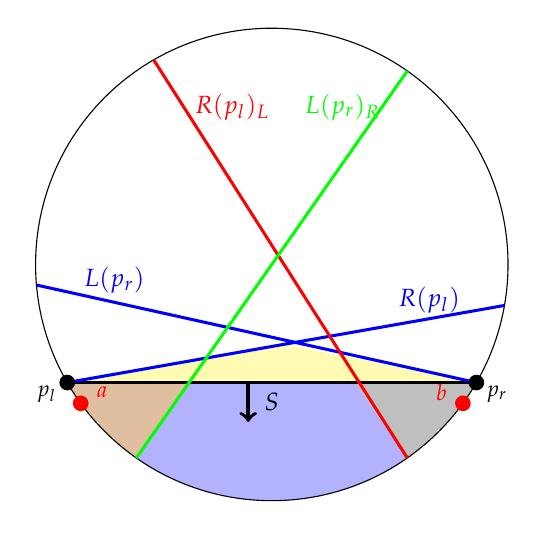
\begin{tikzpicture}
		\fill [color=brown!50] (210:3) -- (-1.05,-1.5) -- (235:3) arc (235:210:3);
		\fill [color=gray!50] (305:3) -- (1.05,-1.5) -- (330:3) arc (330:305:3);
		\fill [color=yellow!30] (210:3) -- (0.1,-1) -- (330:3);
		\fill [color=blue!30] (235:3) -- (-1.05,-1.5) -- (1.05,-1.5) -- (305:3) arc (305:235:3);
		\draw (0,0) circle (3);
		\draw [color=black,line width=1.1pt] (210:3) -- node [below] {\small$S$} (330:3);
		\draw [color=black,line width=1.3pt,->] (-0.3,-1.5) -- +(0,-0.5);
		\draw [color=blue,line width=1.1pt] (185:3) -- (330:3)
		(210:3) -- (350:3);
		\draw [color=red,line width=1.1pt] (120:3) -- (305:3);
		\draw [color=green,line width=1.1pt] (55:3) -- (235:3);
		\node [color=blue] at (-2,-0.2) () {\small$L(p_r)$};
		\node [color=blue] at (2,-0.45) () {\small$R(p_l)$};
		\node [color=red] at (-0.5,2) () {\small$R(p_l)_L$};
		\node [color=green] at (0.9,2) () {\small$L(p_r)_R$};
		\node [color=red,fill=red,circle,inner sep=2] at (216:3) () {};
		\node [color=red,fill=red,circle,inner sep=2] at (324:3) () {};
		\node at (210:3.3) () {\footnotesize $p_l$};
		\node [color=black,circle,fill,inner sep=2] at (210:3) () {};
		\node at (330:3.3) () {\footnotesize $p_r$};
		\node [color=black,circle,fill,inner sep=2] at (330:3) () {};
		\node [color=red] at (217:2.7) () {\footnotesize $a$};
		\node [color=red] at (323:2.7) () {\footnotesize $b$};
	\end{tikzpicture}
	\caption{Here we have a set $S$ which is crossed on both sides. We use in \cref{lem:circsubset} that $L(p_r) \cap R(p_l) = S$; in other words, the yellow region is empty.}
\end{figure}


\circsubset*
\begin{proof}
	For convenience, let $L=L(p_r)$ and $R=R(p_l)$. First suppose we had $L = S$ or $R = S$. In this case, by definition $E^\circ(S) = E^\circ(L)$ or $E^\circ(R)$, and we are done. So assume that $S \subsetneq L, R$. Therefore, $L$ and $R$ cross.  
	
	Now, notice that since $O(L \cap R) = O(S)$, by \cref{lem:extendedprop20}, we have $L \cap R = S$. This implies
	$\delta(S) \subseteq \delta(L) \cup \delta(R)$. To see this, let $e$ be an edge in $\delta(S)$. Then, it has an endpoint in both $L$ and $R$. However, its other endpoint is in $\overline{S} = \overline{L \cap R}$, and therefore cannot be in both $L$ and $R$ which implies it is in $\delta(L)$ or $\delta(R)$.  

	Now, by way of contradiction, suppose there exists an edge $e \in E^\circ(S)$ such that $e \not\in E^\circ(L) \cup E^\circ(R)$. Since $E^\leftarrow(S) = E^\leftarrow(R)$, $E^\rightarrow(S) = E^\rightarrow(L)$, and $e \in \delta(L) \cup \delta(R)$, it must be that $e \in E^\leftarrow(L) \cup E^\rightarrow(R)$. Since $L$ and $R$ cross, by \cref{cor:leftrightemptyextended} $e$ is in exactly one of $E^\leftarrow(L),E^\rightarrow(R)$; assume that $e \in E^\leftarrow(L)$ but not in $E^\rightarrow(R)$, the other case is similar. Therefore $e \not\in \delta(R)$, since it is not in $E^\leftarrow(R), E^\circ(R)$ or $E^\rightarrow(R)$. 
	
	However, $L_L$ crosses $L$ on the left and $R$ crosses $L$ on the right. Therefore, by \cref{lem:nointersectionLR}, we have $(L_L \smallsetminus L) \cap (R \smallsetminus L) = \emptyset$. However $e$ has one endpoint in $L \cap R = S$, one in $R \smallsetminus L$ (since $e \not\in \delta(R), e \in \delta(L)$), and one in  $L_L \smallsetminus L$, which is a contradiction since all three sets are disjoint. 
\end{proof}




\subsection{Every cut is mapped to a constant number of bad events}

In this section we prove \cref{lem:constant-num-events}. 

\constantnumberevents*
\begin{proof}
First note that by \cref{fact:union-not-everything}, $O(L(p) \cup L(q)) \not= O(\cA(\cC))$, so it forms a contiguous interval. WLOG assume that $q$ is the rightmost point in this interval.   

Suppose by way of contradiction that $e \in E(B^\rightarrow(p)) \cap E(B^\rightarrow(q))$	. In the below claim, we will show that $L(p)_R$ crosses $L(q)$ on the right. Now we will show that $L(p)$ crosses $L(q)^{\cap R}$ on the left, which would complete the proof. This is because $L(p)$ is a candidate for $L^*(q)$, and by \cref{lem:crosschain}, $L(p) \cap L(q)^{\cap R} \subseteq L^*(q) \cap L(q)^{\cap R}$, which implies $a \in L^*(q)$ and therefore we could not have $e \in E(B^\rightarrow(q))$. 

It remains to show that $L(p)$ crosses $L(q)^{\cap R}$ on the left. By assumption, $a \in L(p) \cap L(q)^{\cap R}\not= \emptyset$. $L(q)$'s rightmost atom is in $L(q)^{\cap R} \smallsetminus L(p)$. So it remains to show that $L(p) \not\subseteq L(q)^{\cap R}$. By way of contradiction suppose $L(p) \subseteq L(q)^{\cap R} = L(q) \cap L(q)_R$. Since by the following claim, $L(p)_R$ crosses $L(q)$ on the right, $L(p)_R$ is a candidate for $L(q)_R$. We will show that $|O(L(p)_R \cap L(q))| < |O(L(q)_R \cap L(q))|$ which contradicts \cref{def:SLR}. Since $L(p)_R$ and $L(q)_R$ both cross $L(q)$ on the right, to prove the inequality it's enough to show that the leftmost outside atom of $L(q)_R$ is not in $L(p)_R$. However, this is immediate because $L(p)_R$ does not have the leftmost outside atom of $L(p)$, yet $L(p) \subseteq L(q)^{\cap R}$. 
%However, the leftmost outside atom of $L(p)$ is not in $L(p)_R$ but it is in $L(q)_R$, which is a contradiction since $L(q)_R$ minimizes the number of outside atoms in the intersection. 
\begin{claim}
$L(p)_R$ crosses $L(q)$ on the right.
\end{claim}
\begin{proof}
First we show that $L(p)_R$ crosses $L(q)$. Note $b \in L(p)_R \smallsetminus L(q)\not=\emptyset$, and $a \in L(p)_R \cap L(q) \not=\emptyset$. So, $L(p)_R$ crosses $L(q)$ unless $L(q) \subseteq L(p)_R$.  For contradiction, assume $L(q) \subseteq L(p)_R$. %and similarly $L(p) \subseteq L(q)_R$. 

Now we claim that $L(p)$ crosses $L(q)$. By assumption, $a \in L(p) \cap L(q)$. $L(q) \subseteq L(p)_R$ implies $L(p) \not\subseteq L(q)$. Since $q$ is the rightmost point of the interval $O(L(p) \cup L(q))$, the rightmost atom of $L(q)$ is in $L(q) \smallsetminus L(p)$, giving $L(q) \not\subseteq L(p)$. Therefore, $L(q)$ crosses $L(p)$ on the right. 

Therefore, $L(q)$ is a candidate set for $L(p)_R$, but since $L(q) \subseteq L(p)_R$, we must have $L(q) = L(p)_R$. Yet $b \in L(p)_R \smallsetminus L(q)$ which contradicts this.

Now we establish that $L(p)_R$ crosses $L(q)$ \textit{on the right}. For contradiction, suppose it crosses on the left. Then, by \cref{lem:nointersectionLR}, we must have $(L(p)_R \smallsetminus L(q)) \cap (L(q)_R \smallsetminus L(q)) = \emptyset$, which contradicts the fact that $b$ lies in both sets. 
\end{proof} 
\end{proof}

%\begin{lemma}\label{lem:small-exp-cost-both-sides}
%For all edges $e$,
%	$$\E{s^*_e} \le 13\alpha\eta x_e$$
%\end{lemma}
%\begin{proof}
%Fix an outside atom $a$. using (1), (2), and (3) from \cref{obs:L(a)capr} together with \cref{lem:treeoneedge} implies that $$\P{E^\Rightarrow(L(a)))_T = 1} \ge 1-\frac{3+2+2}{2}\eta= 1-\frac{7}{2}\eta.$$ 
%%The same holds for $E^\Leftarrow(R(a))$. 
%
%Secondly, by (4) of \cref{obs:L(a)capr}, $x(E^\Rightarrow(L(a))),x(E^\Leftarrow(L(a)))\geq 1-\eta$. So, since $L(a)$ is an $\eta$-near mincut by \cref{lem:ERLOpartition}, $x(E^\circ(L(a))) \le 3\eta$.
%So $\P{E^\circ(L(a))_T=0} \geq 1-3\eta$ by \cref{fact:0edgerandomspanningtree}. %(similarly for $E^\circ(R(a_i))$). 
%Putting these together, by union bound,
%$$ \P{E^\Rightarrow(L(a))_T=1,  E^\circ(L(a))_T=0} \geq 1-\frac{13}{2}\eta.$$
%
%Now, fix an edge $e$. This edge is in at most one polygon, and by \cref{lem:edgein2sets}, there is at most one (outside) atom $a$ such that $e\in E^\Rightarrow(a)$. That means that the probability that $e$ increases due to a right increase event is at most $13\eta/2$. Recall that in such a case we define $s^*_e=\alpha x_e$.
%Similarly, the probability that $e$ increases due to a left increase event is at most $13\eta/2$.
%Putting these together, we get $\E{s^*_e}=\alpha x_e \cdot \frac{13\eta}{2} + \alpha x_e\cdot \frac{13\eta}{2}=13\alpha\eta x_e$ as desired. 
%\end{proof}




%\subsection{Proof of \cref{thm:cutsbothsideswithinside}}%\label{sec:poly}



%\begin{figure}[htb]\centering
%	\begin{tikzpicture}
%		\fill [color=blue!30] (240:3) -- (0.03,-1.61) -- (280:3)  arc (280:240:3); 
%		\fill [color=yellow!30] (280:3) -- (0.03,-1.61) -- (1.1,-0.88) -- (330:3) arc (330:280:3);
%		\fill [color=orange!30] (330:3) -- (1.1,-0.88) -- (5:3) arc (365:330:3);
%		\draw (0,0) circle (3);
%		\draw [color=green,line width=1.1pt] (240:3) -- (5:3);
%		\node [color=green] at (2,0.3) () {\small$L(b)_r$};
%		\draw [color=red, line width=1.1pt] (170:3) --   (330:3);
%		\node [color=red] at (-2,0.5) () {\small$L(b)$};
%		\draw [color=blue,line width=1.1pt] (120:3) -- (280:3);
%		\node [color=blue] at (-0.3,2) {\small$(L(b)^{\cap r})_L$};
%
%		\node [draw,circle,fill=black,] at (323:3) {};
%		\node at (323:3.5) () {$b$};
%	\end{tikzpicture}
%	\caption{An Illustration of \cref{defn:LaRbetc}. Here the polygon is represented by a circle. The edges in $E^\Rightarrow(b)$ have one endpoint in yellow and one endpoint in orange region. Note that the $L(b)_r$ is chosen to minimize the number of atoms in the regions blue and yellow. $(L(b)^{\cap r})_L$ is chosen to maximize the number of atoms in the blue region. }
%	\label{fig:Rightarrowdef}
%\end{figure}
%
%
%\begin{figure}[htb]\centering
%	\begin{tikzpicture}
%		\fill [color=brown!50] (210:3) -- (-1.05,-1.5) -- (235:3) arc (235:210:3);
%		\fill [color=gray!50] (305:3) -- (1.05,-1.5) -- (330:3) arc (330:305:3);
%		\fill [color=yellow!30] (-1.05,-1.5) -- (0.1,0.2) -- (1.05,-1.5) -- (-1.05,-1.5);
%		\fill [color=blue!30] (235:3) -- (-1.05,-1.5) -- (1.05,-1.5) -- (305:3) arc (305:235:3);
%		\draw (0,0) circle (3);
%		\draw [color=black,line width=1.1pt] (210:3) -- node [above] {\small$S$} (330:3);
%		\draw [color=blue,line width=1.1pt] (185:3) -- (330:3)
%		(210:3) -- (350:3);
%		\draw [color=red,line width=1.1pt] (120:3) -- (305:3);
%		\draw [color=green,line width=1.1pt] (55:3) -- (235:3);
%		\node [color=blue] at (-2,-0.2) () {\small$L(b)$};
%		\node [color=blue] at (2,-0.45) () {\small$R(a)$};
%		\node [color=red] at (-0.5,2) () {\small$R(a)_l$};
%		\node [color=green] at (0.9,2) () {\small$L(b)_r$};
%		\node [draw,fill=black,circle,inner sep=1mm] at (216:3) () {};
%		\node [draw,fill=black,circle,inner sep=1mm] at (324:3) () {};
%		\node  at (217:3.5) () {$a$};
%		\node  at (323:3.5) () {$b$};
%	\end{tikzpicture}
%	\caption{Setting of \cref{lem:ERLOpartition}. In the lemma we prove that $R(a)_l\cap L(b)_r\subseteq S$, thus the yellow region
%	is empty. Note that another possible way to observe the yellow region is empty is to use \cref{thm:halfplanes}.}
%	\label{fig:E(S)partition}
%\end{figure}




%\subsection{Happy Polygons}
%\label{sec:happypolygons}


\section{Putting everything together}\label{sec:hierarchy}
 
%In this section we will combine \cref{thm:crossed-one-side} and \cref{thm:cutsbothsideswithinside} with one of the main results from ~\cite{KKO21} to prove \cref{thm:main}. We note that this section, similar to the proof of \cref{thm:crossed-one-side}, is not conceptually different from ~\cite{KKO21}.

In this section we use the following theorem to demonstrate \cref{thm:main}. While the proof of \cref{thm:maintechnical} is non-trivial, using \cref{thm:cutsbothsideswithinside} it follows from statements in \cite{KKO21} and does not require any new ideas. For this reason, we sketch the proof in this section, leaving the formal proof to \cref{app:proofbeforetechnical}. 

It turns out not to be useful to prove \cref{thm:hierarchyKKO} directly, but is an immediate corollary of the following theorem (we stated \cref{thm:hierarchyKKO} in the overview to improve readability and highlight the importance of \cref{thm:cutsbothsideswithinside}).

%One can see this theorem as a combination of \cref{thm:cutsbothsideswithinside} and \cref{thm:hierarchyKKO}, where the latter is a combination (and slight modification) of two theorems in \cite{KKO21}. Note we do not formally prove \cref{thm:hierarchyKKO} in this paper in order to more closely follow the proof template of \cite{KKO21}; it is instead used to help give intuition in the \cref{sec:overview}. However it can be proved in a nearly identical manner to the below by simply ``leaving out" the slack vector constructed in \cref{thm:cutsbothsideswithinside}. 

%The main goal of the section will be to show the following theorem. We set . 

\begin{restatable}[Combination of \cref{thm:hierarchyKKO} and \cref{thm:cutsbothsideswithinside}]{theorem}{maintechnical}\label{thm:maintechnical}
Let $x^0$ be a solution of LP \eqref{eq:tsplp} with support $E_0=E\cup \{e_0\}$, and $x$ be $x^0$ restricted to $E$.
Let $\eta\leq 10^{-12}, \decrease > 0$ and let $\mu$ be  the max-entropy distribution with marginals  $x$. 
Then there are two functions $s: E_0\rightarrow \R$ and $s^*: E \rightarrow \R _{\ge 0}$ (as functions of $T\sim\mu$), such that
\begin{enumerate}[i)]
\item For each edge $e \in E$, $s_e \ge -x_e \decrease$ (with probability 1). 
\item
For each $S \in \cN_{\eta}$, if $\delta(S)_T$ is odd, then
$  s(\delta(S)) + s^*(\delta(S)) \ge  0.$
\item For every edge $e$, $\E{s^*_{e}}\leq 125\eta \decrease x_e$ and $\E{s_e}\leq -\frac{1}{3}x_e \eps_P\decrease $, where $\eps_P$ is defined in \cref{thm:payment-main}.      
\end{enumerate}
\end{restatable}

In \cref{subsec:proofofmain} we show how this theorem implies \cref{thm:main}. Now we sketch the ideas underlying the proof of \cref{thm:maintechnical}. To make this section as accessible as possible, we  oversimplify and ignore the details of how parameters are set.

In the above theorem, the role of $s$ is to generate gain over $3/2$. Roughly speaking, we follow the lead of \cite{KKO21} and divide $\cN_\eta$ into three categories: cuts crossed on both sides, cuts crossed on one side, and the remainder, which form a laminar family $\cH$ defined below. We define an $s^*$ vector to provide significant positive slack on each odd cut that is crossed; in particular, we  start with the vector defined in \cref{thm:cutsbothsideswithinside} and augment it to handle cuts crossed on one side. We will ensure that the expected cost of $s^*$ is negligible\footnote{i.e., $\E{s^*_{e}} \leq 18\alpha\eta x_e$, which will ultimately be $O(\eta \decrease x_e)$. In the end, this increase is dwarfed by a \textit{decrease} in $s_e$ of $\Omega(\decrease x_e )$ since $\eta$ is a minuscule constant.}. Now in $\cH$, there are only a linear number of cuts and they have a simple structure (for example, most edges are only in a constant number of cuts of $\cH$), so it is manageable to design a vector $s$ which generates negative slack in expectation while still satisfying every cut in $\cH$. 

%\cref{thm:cutsbothsideswithinside} shows that at negligible expected cost we can ensure that $s^*$ provides significant positive slack on each odd cut crossed on both sides. This guarantees that even if all edges have $s_e$ reduced (negative) as per the discussion later in this section, every cut crossed on both sides will still be satisfied in the $O$-join.

%It remains to satisfy the  cuts in $\cN_{\eta,\le 1}$, while simultaneously ensuring that $\E{s_e}$ is sufficiently negative on each edge. To do this, we will need to further augment the $s^*$ vector from \cref{thm:cutsbothsideswithinside}.

First, we explain how to augment $s^*$ from \cref{thm:cutsbothsideswithinside} to handle cuts crossed on one side. Observe that any polygon associated to a connected component in $\cN_{\eta,\le 1}$ contains no inside atoms. This follows  from the fact that the existence of an inside atom is predicated on the existence of a $k$-cycle, which by its very definition  contains cuts crossed on both sides. Thus, each connected component $\cC$ of $\cN_{\eta,\le 1}$ consists only of outside atoms, where $a_0$ is the root.

A key structure needed for the construction of the slack vector $s$ is a laminar family of cuts $\cH$ that we call a {\em hierarchy}. This hierarchy $\cH$ includes the following set of cuts:
\begin{itemize}
\item The set of cuts in $\cN_{\eta, \le 1}$ that are not crossed by any other cut in  $\cN_{\eta, \le 1}$;
\item The cut consisting of the union of the non-root atoms $\{a_1, \ldots, a_{m-1}\}$ of each 	connected component $\cC$ of $\cN_{\eta, \le 1}$, which (in this section) we call the {\em outer polygon cut} for  $\cC$, and
\item The atoms $a_i$, $1\le i \le m-1$ of each connected component $\cC$ of $\cN_{\eta, \le 1}$.
\end{itemize}

Notice that $\cH$ {\em excludes} some cuts in $\cN_{\eta, \le 1}$, namely all the near min cuts in any polygon $P$ of $\cN_{\eta, \le 1}$ that are {\em not} outer polygon cuts.
It also {\em includes} some cuts that are {\em not} in $\cN_{\eta, \le 1}$. For example, the outer polygon cut itself may not be an $\eta$ near min cut, and there may be atoms in some polygon that are not $\eta$ near min cuts.
However, one of the consequences of the following theorem is that these extra cuts  are $\eps_\eta$ near min cuts where $\eps_{\eta}= 7\eta$:
%\footnote{The main observation used to prove \cref{thm:approxpoly} is that the cuts in a single connected component  $\cC$ of $ \cN_{\eta,1}$ can be partitioned into two laminar families $\cL$ and $\cR$, where $\cL$ (resp. $\cR$) is the set of cuts crossed on the left (resp. right).
%This immediately implies that $|\cC|$ is linear in $m$. Since cuts in $\cL$ cannot cross each other (and similarly for $\cR$), the proof boils down to understanding the interaction between $\cL$ and $\cR$.} 


%This means that there are four types of cuts remaining that we will be interested in (as always, assuming the root is in $\overline S$):
%\begin{itemize}
%\item {\em Degree cuts}: these are cuts which are not crossed by any other cut in $\cN_{\eta,\le 1}$. The simplest type of degree cut is a vertex cut.
%\item {\em Triangle cuts}: A triangle cut $S = a_1 \cup a_2$ is a cut that is the union of two disjoint near min cuts $a_1$ and $a_2$. (For a triangle cut, we will use $a_0$ to denote $\overline S$.)
%\item {\em Outer polygon cuts}: These are the cuts $S=\{a_1, \ldots, a_{m-1}\}$ where $a_1, \ldots, a_{m-1}$ are the non-root atoms of some polygon $P$ of $\cN_{\eta,\le 1}$;.
%\item {\em Cuts crossed on one side} (that are not an outer polygon cut): These  cuts are defined by a contiguous interval of non-root atoms $\{a_i, a_{i+1}, a_j \}$, for $ i\le j$  in some polygon $P$ of $\cN_{\eta,\le 1}$.
%\end{itemize}
%
%
%We use the following theorem:
\begin{theorem}[Structure of Polygons of $\cN_{\eta, 1}$ (Theorem 4.9 from \cite{KKO21})]\label{thm:approxpoly}
For  $\eps_{\eta}\geq 7\eta$ and any polygon of $\eta$ near min cuts $\cC$ crossed on one side with atoms $a_0...a_{m-1}$ (where $a_0$ is the root) the following holds:
	\begin{itemize}
	\item For all adjacent atoms $a_i,a_{i+1}$ (also including $a_0,a_{m-1}$), we have $x(E(a_i,a_{i+1})) \ge 1-\eps_\eta$. 
	\item All atoms $a_i$ (including the root) have $x(\delta(a_i)) \le 2+\eps_\eta$. 
	\item $x(E(a_0, \{a_2,\dots,a_{m-2}\}))\leq \eps_{\eta}$.
 %In addition $x(\{a_0...a_{m-1}\}) \le 2+\eps_\eta$. 
	\end{itemize}
\end{theorem}

\cref{thm:approxpoly} shows that polygons of cuts crossed on one side  nearly look like cycles.
Now, if magically it was the case that  $x(E(a_i, a_{i+1 \pmod{m}})) =1$, and $x(\delta(a_i))=2$
for $1 \le i \le m-1$, then with probability 1 (see \cref{lem:treeoneedge}), we would have $E(a_i, a_{i+1})_T = 1$ and we would be able to claim that:  
\begin{itemize}
\item [(i)] any cut in $\cC$ which does not include either $a_1$ or $a_{m-1}$ (and is therefore not in $\cH$) is even in the tree with probability 1; 
\item[(ii)] The  cuts in $\cC$ that contain $a_1$ but not $a_{m-1}$, i.e., the so-called "leftmost cuts" (also not represented in $\cH$) are even precisely when $E(a_0, a_1)_T$ is odd and 
\item [(iii)] the cuts in $\cC$ that contain $a_{m-1}$  but not $a_1$ i.e., the "rightmost cuts", are even when $E(a_0, a_{m-1})_T$ is odd. 
\end{itemize}
\cref{thm:approxpoly} can be used to show that this approximation is 
 correct up to $O(\eta)$. In other words, we augment $s^*_e$ as needed on each edge between adjacent non-root atoms in each connected component $\cC$, at the cost of increasing $\E{s_e^*}$ by an additional (again negligible) $O(\eta\decrease x_e)$. This allows us to pretend our magical thinking is correct. Thus, all of the $\eta$ near min cuts in the polygon that are {\em not} represented in the hierarchy are satisfied so long as the outer polygon cut 
is {\em happy}, that is,  $E(a_0, a_1)_T = E(a_0, a_{m-1})_T = 1$ and $E(a_0, \{a_2, \ldots, a_{m-2}\})_T = 0$.

%Therefore, as long as the outer polygon cut for a polygon is {\em happy}, that is, it holds that $E(a_0, a_1)_T = E(a_0, a_{m-1})_T = 1$ and $E(a_0, \{a_2, \ldots, a_{m-1})_T = 0$ {\em all} the cuts in the polygon are satisfied at small additional cost.  
%
%One can think of a triangle $S$ as a degenerate polygon with three atoms and using reasoning similar to that above, one can argue that so long as the triangle is {\em happy}, that is, $E(a_0, a_1)_T = E(a_0, a_{2})_T = 1$, the cuts $a_1$ and $a_2$ are also satisfied (again, at a possible $O(\eta\decrease)$ expected slack increase on $s^*_e$ for edges $e \in E(a_1, a_2)$).


 %Our main remaining task is to explain how  we use the hierarchy $\cH$ to choose a slack vector $s$ that has {\em negative} expected value, specifically, has $\E{s_e} = -c\eta x_e$ for each edge, where $c$ is large enough that $-\E{s_e} \gg \E{s_e^*}$ for all $e$ and all O-join constraints are satisfied by setting $y_e = 0.5 x_e + s_e + s_e^*$.
 
% \begin{remark} In the statement of \cref{thm:hierarchyKKO}, we fold the increases in $s_e^*$ due to cuts crossed on one side into the definition of $s_e$, thus setting the $s$ of that theorem to be $s+s^*$ from the above discussion.
%\end{remark}
 
 
%  
%\begin{remark} To simplify the exposition in the overview, in the statement of \cref{thm:hierarchyKKO}, we folded the increases in $s_e^*$ due to cuts crossed on one side into the definition of $s_e$.
%\end{remark}


\subsection{Constructing the slack vector $s$} 

%The slack vector $s$ is defined  using a laminar family $\cH$ of near min cuts called a hierarchy\footnote{The hierarchy is the set of cuts consisting of all cuts in $\cN_{\eta, \le 1}$ that are not crossed by any other cut in  $\cN_{\eta, \le 1}$, together with the outer polygon cut and the atoms of each polygon of $\cN_{\eta, \le 1}$.} consisting of all $\eta$-near mincuts of $x$  that are not crossed. These are the degree cuts, the triangle cuts and the outer polygon cuts. 
%See \cref{fig:hierarchywithtriangle} for an example of a hierarchy with three triangles.





\begin{figure}[htb]
	\centering
	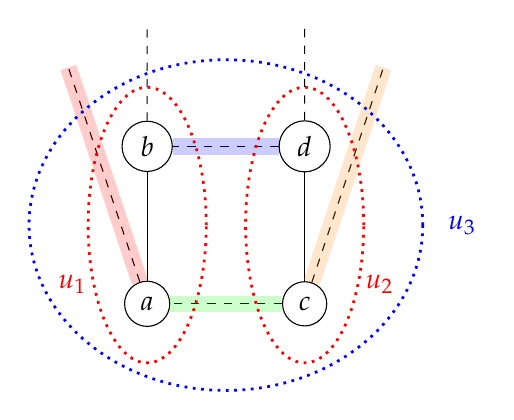
\begin{tikzpicture}
		\node [draw,circle] at (0,0) (a) {$a$};
		\node [draw,circle] at (0,2) (b) {$b$} edge (a);
		\node [draw,circle] at (2,0) (c) {$c$} edge [dashed] (a) edge [color=green,line width=6pt,opacity=0.2] (a) ;
		\node [draw,circle] at (2,2) (d) {$d$} edge (c) edge [dashed] (b) edge [line width=6pt,opacity=0.2,color=blue] (b);
		\draw [dashed] (a) -- +(-1,3)  (b) -- +(0,1.5) (d) -- +(0,1.5) (c) --  +(1,3);
		\draw [color=red,line width=6pt,opacity=0.2] (a) -- +(-1,3);
		\draw [color=orange,line width=6pt,opacity=0.2] (c) --  +(1,3);
		\draw [dotted,line width=1pt, color=red] (0,1) ellipse (0.75 and 1.75)
			(2,1) ellipse (0.75 and 1.75);
		\draw[line width=1pt,dotted,color=blue]	(1,1) ellipse (2.5 and 2.1);
		\node [color=red]at (-0.95,0.25) () {$u_1$};
		\node [color=red] at (2.95,0.25) () {$u_2$};
		\node [color=blue] at (4,1) () {$u_3$};
		
	\end{tikzpicture}
	\quad \quad \quad
	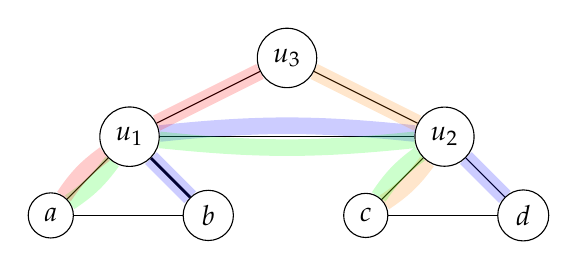
\begin{tikzpicture}
		\node [circle,draw] at (0,0) (a) {$a$};
		\node [circle,draw] at (2,0) (b) {$b$} edge (a);
		\node[circle,draw]  at (1,1) (u1) {$u_1$} edge (a) edge [color=green,opacity=0.2,line width=6pt,bend left=10] (a) edge [opacity=0.2,line width=6pt,color=red,bend right=10] (a) edge [line width=1pt](b) edge [color=blue,opacity=0.2,line width=6pt](b);
		\node[circle,draw]  at (4,0) (c) {$c$};
		\node [circle,draw] at (6,0) (d) {$d$} edge (c);
		\node [circle,draw] at (5,1) (u2) {$u_2$} edge (c) edge [color=orange,line width=6pt,opacity=0.2,bend left=10] (c) edge [color=green,opacity=0.2,line width=6pt,bend right=10] (c) edge (d) edge [color=blue,opacity=0.2,line width=6pt] (d) edge (u1) edge [color=blue,opacity=0.2,line width=6pt,bend right=6] (u1) edge [color=green,opacity=0.2,line width=6pt,bend left=6] (u1);
		\node[circle,draw]  at (3,2) (u3) {$u_3$} edge (u1) edge [color=red,opacity=0.2,line width=6pt] (u1) edge (u2) edge [color=orange,line width=6pt,opacity=0.2] (u2) ;
	\end{tikzpicture}
	\caption{\small An example of part of a hierarchy with three "triangles". The graph on the left shows part of a feasible LP solution where dashed (and sometimes colored) edges have fraction $1/2$ and solid edges have fraction 1. The dotted ellipses on the left show the min-cuts $u_1,u_2,u_3$ in the graph. (Each vertex is also a min-cut). On the right is a representation of the corresponding hierarchy. Triangle $u_1$ corresponds to the cut $\{a,b\}$, $u_2$ corresponds to $\{c,d\}$ and $u_3$ corresponds to $\{a,b,c,d\}$. Note that, for example, the edge $\{a,c\}$, represented in green,  is in $\delta(u_1)$,  $\delta(u_3)$, and inside $u_3$. In this example, $\p (\{a,b\}) = u_1$ and  $\p (\{a,c\}) = u_2$. Triangle $u_1$ is happy if $(\delta(a)\smallsetminus \{a,b\})_T = (\delta(b)\smallsetminus \{a,b\})_T = 1$.  }
	\label{fig:hierarchywithtriangle}
\end{figure}


 


 Our main remaining task is to explain how to use the hierarchy $\cH$ to choose a slack vector $s$ that has {\em negative} expected value, specifically, has $\E{s_e} = -\Omega(\decrease x_e)$ for each edge, while ensuring that all $O$-Join constraints coming from $\cH$ are satisfied. %Therefore by the above arguments, combining $s_e$ and $s_e^*$ ensures that \textit{all} constraints coming from $\cN_{\eta}$ are satisfied, and moreover since $-\E{s_e} \gg \E{s_e^*}$ we have $\E{s_e + s^*_e}$ sufficiently negative for $\eta$ small enough.

 %We now briefly review how \cite{KKO21} used the hierarchy and the sampled tree to construct a good slack vector $s$. 
 As mentioned in \cref{sec:overview}, the approach taken is to set $s_e$ to be negative (i.e. {\em reduce} it) when certain special cuts $e$ is on are even in the tree and therefore induce no $O$-join constraint. Roughly speaking, it works as follows: For each LP edge $f$, consider the lowest cut $S$ in the hierarchy that contains both endpoints of $f$. We call this cut $\p(f)$ (for "parent of $f$").
  Let $\bbe = \{u,v\}$ (where $u$ and $v$ are children of $S$ in $\cH$; recall $u,v$ are subsets of vertices) be the set of all edges $f = \{u', v'\}$ such that $u' \in u$ and $v' \in v$. 
  
 Cuts in $\cH$ are separated into three types. If $S \in \cH$ has at least three children and it is not an outer polygon cut, call it a \textit{degree cut}. If it has exactly two children, call it a \textit{triangle cut}. The remaining cuts, as defined above, are outer polygon cuts.

 If $\p(f)$ is a degree cut, then  set $s_f :=  - 0.57\decrease x_f$ for all $f \in \bbe$ whenever the event that $\delta(u)_T$ and $\delta(v)_T$ are both even in the tree occurs. Call $f$ ``good" if this event occurs with constant probability. Furthermore, it is shown that every cut $u$ with $\p(u)$ a degree cut contains a $\Omega(1)$ fraction of good edges.
% It is shown that for every cut $u$ (with $\p(u)$ a degree cut), the probability of this good event is $\Omega(1)$ for a subset of ``good" edges $G \subseteq \delta(S)$ where $x(G) \ge \Omega(1)$. 
 
 On the other hand, when $\p(f)$ is an outer polygon cut or a "triangle" cut (see \cref{fig:hierarchywithtriangle}), set $s_f = -  \decrease x_f$ for all $f \in \bbe$ whenever $p(f)$ is happy (as defined above).   Thus, when a polygon  is happy, {\em all} edges $e$ whose parent is that cut have their slack $s_e$ reduced simultaneously. %(and at an expected cost of $O(\eta\decrease x_e)$ per edge, all near min cuts internal to the polygon are simultaneously satisfied). 
 Moreover, the event that $p(f)$ is happy for a polygon cut (or triangle cut) occurs with constant probability.
    
However, regardless of the type of cut $p(f)$ is,   setting $s_f$ to a negative value can be problematic for the feasibility of other cuts lower down in the hierarchy that contain $f$. Therefore, when a cut $S'$ lower down in the hierarchy such that $f \in \delta(S')$ is  odd in the tree, the slack of {\em other} edges  in $\delta(S')$ are increased to compensate for the reduction in $s_f$, (i.e., to maintain feasibility of $y$ for the cut $S'$). 
 
 The challenge is to do all of this in a way that still guarantees that  overall $\E{s_e} < - \eps \decrease x_e$, while simultaneously ensuring that for any cut $S \in \cH$ if $\delta(S)_T$ is odd, $\sum_{e \in \delta(S)} s_e \ge 0$. Showing this is involved and requires careful probabilistic arguments that rely on the fact that the tree is sampled from a max-entropy distribution. We refer the reader to \cite{KKO21} for the details.
 
 %$S \in \cN_{\eta,\le 1}$, if $\delta(S)_T$ is odd, $\sum_{e \in \delta(S)} (s_e + s_e^*) \ge 0$. 
 
 
 \subsection{Proof of \cref{thm:main} using \cref{thm:maintechnical}}\label{subsec:proofofmain}

\maintechnical*
%Here we show how our main theorem follows easily from \cref{thm:maintechnical}:
\begin{proof}[Proof of \cref{thm:main}]
Let $x^0$ be an extreme point solution of LP \eqref{eq:tsplp}, with support $E_0$ and let $x$ be $x^0$ restricted to $E$. By \cref{fact:sptreepolytope} $x$ is in the spanning tree polytope. 
Let $\mu=\mu_{\lambda^*}$ be the max entropy distribution with marginals $x$, and let $s,s^*$ be as defined in \cref{thm:maintechnical}.
We will define $y:E_0\to\R_{\geq 0}$ such that:
$$y_e=\begin{cases}
x_e/2+s_e+s^*_e & \text{if } e\in E\\
\infty & \text{if } e=e_0
\end{cases}
$$	
We will show that $y$ is a feasible solution
to \eqref{eq:tjoinlp}.
First, observe that for any $S$ where $e_0\in\delta(S)$, we have $y(\delta(S))\geq 1$. Otherwise, we assume $u_0,v_0\notin S$.
If $S$ is an $\eta$-near min cut and $\delta(S)_T$ is odd, then by property (ii) of \cref{thm:maintechnical}, we have
$$ y(\delta(S)) = \frac{x(\delta(S))}{2}+ s(\delta(S))+s^*(\delta(S))\geq 1.$$
On the other hand, if $S$ is not an $\eta$-near min cut, then
$$y(\delta(S)) \geq (\frac{1}{2}-\decrease)x(\delta(S)) \ge (\frac{1}{2}-\decrease) \cdot (2+\eta) = 1+\frac{\eta}{2}-2\decrease -\decrease \eta$$
where in the first inequality we used property (i) of \cref{thm:maintechnical} which gives $s_e\geq -x_e \decrease$ with probability 1 along with the fact that $s^*$ is non-negative.
Therefore, choosing $\beta = \frac{\eta}{4+2\eta}$ ensures that $y$ is a feasible $O$-join solution.

Finally, using $c(e_0)=0$ and part (iii) of \cref{thm:maintechnical},
\begin{align*}
\E{c(y)}&= c(x)/2 + \E{c(s)} +\E{c(s^*)}\\
&\leq c(x)/2 - \eps_P \decrease \cdot \frac{1}{3}c(x) +125\eta \cdot \decrease  \cdot c(x)\\
&\leq (1/2-\frac{1}{6}\eps_P\decrease) \cdot c(x)
\end{align*}
choosing $\eta$ such that 
\begin{equation}\label{eq:whatiseta}
 	125\eta= \frac{1}{6}\eps_P
 \end{equation}

Now, we are ready to bound the approximation factor of our algorithm.
First, since $x^0$ is an  extreme point solution of \eqref{eq:tsplp}, $\min_{e\in E_0} x^0_e\geq \frac{1}{n!}$. So, by \cref{thm:maxentropycomp}, in polynomial time\footnote{Since the claim that the integrality gap is bounded below $3/2$ does not depend on the running time, it may appear that this step is unnecessary. However, we need to discuss the running time here because we are giving a stronger result that the max entropy algorithm returns a solution of expected cost at most $(3/2-\eps)c(x)$ in polynomial time.} we can find $\lambda:E\to\R_{\geq 0}$ such that for any $e\in E$, $\PP{\mu_\lambda}{e}\leq x_e(1+\delta)$ for some $\delta$ that we fix later. It follows that
$$ \sum_{e\in E} |\PP{\mu}{e} - \PP{\mu_{\lambda}}{e}| \leq n\delta.$$
By stability of maximum entropy distributions (see  \cite[Thm 4]{SV19} and references therein), we have that $\norm{\mu-\mu_\lambda}_1\leq O(n^4\delta)=:q$. Therefore, {for some $\delta \ll n^{-4}$ we get} $\norm{\mu-\mu_{\lambda}}_1=q\leq \frac{\eps_P\eta}{100}$. That means that 
$$ \EE{T\sim\mu_{\lambda}}{\text{min cost matching}} \leq \EE{T\sim\mu}{c(y)}+  q (c(x)/2) \leq \left(\frac12-\frac{1}{6}\eps_P\decrease 
 + \frac{\eps_P \eta }{100}\right)c(x), $$
where we used that for any spanning tree the cost of the minimum cost matching on odd degree vertices is at most $c(x)/2$.
Finally, since $\EE{T\sim\mu_\lambda}{c(T)}\leq c(x)(1+\delta)$, $\eps_P=3.12\cdot 10^{-16}$, and $\eta=4.16 \cdot 10^{-19}$ (from \eqref{eq:whatiseta}) and $\decrease = \eta/(4+2\eta)$, we get a $3/2-10^{-36}$ approximation algorithm (compared to $c(x)$).
\end{proof}




%The TAI formalization above gives rise to multiple hierarchies of
tentacular agents.  We discuss some of the these below.



\begin{small}
\begin{enumerate}
\item[\textbf{Syntactic Goal Complexity}] The goal $g$ can range in
  complexity from simple propositional statements,
  e.g. $clean{Kitchen}$, to first-order statements.  e.g.
  $\forall r:\mathsf{Room}: clean(r)$, and to intensional statements
  representing cognitive states of other agents
  $$\believes(a, now, \believes(b, now,\forall r: clean(r)))$$

  %%TODO: Make more precise

\item[\textbf{Goal Variation}] According to the definition
  above, an agent $a$ qualifies as being tentacular if it plans for
  just one goal $g$ in tentacular fashion as laid out in the
  conditions above. We could have agents that plan for a number of
  varied and different goals in tentacular fashion. 

  %%TODO: Make more precise

\item[\textbf{Plan Complexity}] For many goals, there will usually be
  multiple plans involving different actions (with different costs and
  resources used) and executed by different agents. 

  %%TODO: Make more precise



\end{enumerate}
\end{small}


%%++++++++++++++++++++++++++++++++++++++++++++++++++++++++++++++++++++
\begin{figure}[h!]
 \centering
 {
  \includegraphics[width=\linewidth]{./TAIagents.pdf}}
 \caption{Pictorial Overview.  \textit{A bit of explanation: That some
     agents are within agents indicates that the outer agent knows
     and/or believes everything relevant about the inner agent; hence
     as agents are increasingly cognitively powerful, the depth of
     their epistemic attitudes grows (reflected in formulae with
     iterated belief/knowledge operators).  Agents grow in
     size/intelligence in lockstep with the logical calculi upon which
     they are based increasing in expressivity and reasoning power;
     $\mathcal{L}_0$ is zero-order logic, $\mathcal{L}_1$ is
     e.g.\ first-order logic, and the particular cognitive calculus
     $\mathcal{DCEC}$ is shown.  Rotation indicates simply that,
     through time, agents perceive and act.}}
 \label{fig:pictorial_overview}
\end{figure}
%%++++++++++++++++++++++++++++++++++++++++++++++++++++++++++++++++++++

%%% Local Variables:
%%% mode: latex
%%% TeX-master: "main"
%%% End:


\section{Conclusion}
In addition to the obvious question of improving the bound proved in this paper, we conclude with some additional  questions.
\paragraph{Open Directions Related to Structure of Near Min Cuts.}
Given a fractionally 2-edge connected graph $G$ let $\cN_\eta$ be the set of $\eta$-near min cuts of $G$. 
Let $\C$ be a connected component of $\cN_\eta$ with $|\C|>2$ with corresponding polygon $P$.

\begin{itemize}
\item Although \cref{thm:uncrossing} characterizes the edges of $G$ w.r.t. $P$ to some extent, we are still far from a perfect characterization. We find the following question illuminating in this direction: perhaps for sufficiently small $\eta$, is it true that for any cut $S\in \C$, $x(E(S, I(P))\leq O(\eta)$, where $I(P)\subseteq \cA(P)$ is the set of inside atoms of $P$?
\item Is there a compact representation of all $2/3$-near mincuts \cite{BG08,Goe21}? (This is a natural target as $2/3$ is the limit $\alpha$ where the number of $\alpha$-mincuts is 
always at most ${n\choose 2}$ in a graph with $n$ vertices; see \cite{GR95}.)
%\item Is there a laminar family over $\cA(P)$, i.e., the leaves of the family are $\cA(P)$ such that 
%\begin{enumerate}[i)]
%	\item For every $S$ in the family $S$ is a disjoint union of its children
%	\item For every $S$ in the laminar family (which is not the root of the family) with children $S_0,\dots,S_{k}$ for some $k\geq 2$, perhaps after renaming, we have $x(E(S_i,S_{i+1})\geq 1-O(\eta)$ for $0\leq i<k$.
%	\item If root of the laminar family has children $S_0,dots,S_k$ then $x(E(S_i,S_{i+1\text{ mod } k+1}))\geq 1-O(\eta)$ for all $0\leq i\leq k$.
%\end{enumerate}
\end{itemize}


\paragraph{Open Directions Related to TSP.}

\begin{enumerate}
\item Since this analysis does not depend on the integral optimum Hamiltonian cycle (in contrast with \cite{KKO21}), the following now appears more approachable: is it possible to de-randomize the max entropy algorithm and obtain a deterministic $3/2-\eps$ approximation for metric TSP?
One path to solving this problem leads to the following question: is it possible to design an efficient algorithm that outputs  a convex combination of at most \textit{polynomially} many spanning trees such that their expected cost is at most OPT and the expected cost of the minimum matching on their odd degree vertices is at most $(1/2-\eps)OPT$?
\item As we discussed in  \cref{sec:overview}, in our analysis first we ``satisfy'' cuts crossed on both sides by choosing a random slack vector.
Then, we delete these cuts and look at the hierarchy of cuts crossed on at most one side, $\cN_{\eta,\leq 1}$, and design another slack vector for every connected component of crossed cuts in $\cN_{\eta,\leq 1}$. The remaining cuts form a hierarchy as we defined in  \cref{app:proofbeforetechnical}. Unfortunately, working with this structure is not identical to satisfying a laminar family of cuts. For one, we do not guarantee that $x$ has no near minimum cuts not given in the hierarchy: we simply show that if they exist, they can be ignored in the constraints of the $O$-Join. This limitation seems to prevent the use of more direct combinatorial approaches such as \cite{HN19,GLLM21}.
So, we leave it as an open problem as to whether it is possible to construct a random slack vector for all cuts in $\cN_{\eta,1},\cN_{\eta,2}$ simultaneously. Such a vector would preserve the original structure of near min cuts; thus when focusing on the hierarchy one can assume no other near min cuts exist. The answer to this question may lead to more significant improvements to the approximation ratio for metric TSP.	
\end{enumerate} 

\printbibliography
\section{On Presentations of Pure Braid Groups}\label{appendix:pn}
\citet{bhattacharya2018path} gave a presentation of a homotopy group for path planning with $n$ agents on a plane, which is a pure braid group $P_n$, with the following generators:
\begin{equation}
\left\{u_{i,j/\gamma_{i+1},\ldots,\gamma_{j-1}}\middle|1\leq i<j\leq n,\,\gamma_{i+1},\ldots,\gamma_{j-1}\in\{+,-\}\right\}.
\end{equation}

The relations are as follows.
\begin{itemize}
    \item For $i<j<k$, $\alpha_{i+1},\ldots,\alpha_{j-1}\in\{+,-\}$, and $\beta_{j+1},\ldots,\beta_{k-1}\in\{+,-\}$,
    \begin{equation}
    \begin{split}
    &u_{i,j/\alpha_{i+1},\ldots,\alpha_{j-1}}
    \cdot
        u_{i,k/\alpha_{i+1},\ldots,\alpha_{j-1},-,\beta_{j+1},\ldots,\beta_{k-1}}
        \cdot u_{j,k/\beta_{j+1},\ldots,\beta_{k-1}}\\
        &\cdot u^{-1}_{i,j/\alpha_{i+1},\ldots,\alpha_{j-1}}
    \cdot
        u^{-1}_{i,k/\alpha_{i+1},\ldots,\alpha_{j-1},+,\beta_{j+1},\ldots,\beta_{k-1}} 
        \cdot u^{-1}_{j,k/\beta_{j+1},\ldots,\beta_{k-1}},
    \end{split}
    \end{equation}
    \begin{equation}
    \begin{split}
    &u_{i,j/\alpha_{i+1},\ldots,\alpha_{j-1}}
    \cdot
        u_{i,k/\alpha_{i+1},\ldots,\alpha_{j-1},-,\beta_{j+1},\ldots,\beta_{k-1}}\\
        &\cdot u^{-1}_{i,j/\alpha_{i+1},\ldots,\alpha_{j-1}}\cdot
        u^{-1}_{i,k/\alpha_{i+1},\ldots,\alpha_{j-1},+,\beta_{j+1},\ldots,\beta_{k-1}},
    \end{split}
    \end{equation}
    and
    \begin{equation}\label{eq:p-rel}
    \begin{split}
    &u_{i,k/\alpha_{i+1},\ldots,\alpha_{j-1},-,\beta_{j+1},\ldots,\beta_{k-1}}
        \cdot u_{j,k/\beta_{j+1},\ldots,\beta_{k-1}}\\
    &\cdot u^{-1}_{i,k/\alpha_{i+1},\ldots,\alpha_{j-1},+,\beta_{j+1},\ldots,\beta_{k-1}} 
    \cdot u^{-1}_{j,k/\beta_{j+1},\ldots,\beta_{k-1}}.
    \end{split}
    \end{equation}
\item Let $i,j,i',j'$ be distinct indices with $i<j,\,i'<j',\,i<i'$. Let $\gamma_{i+1},\ldots,\gamma_{j-1}\in\{+,-\}$ and $\gamma'_{i'+1},\ldots,\gamma'_{j'-1}\in\{+,-\}$ be signs.
When $i<i'<j<j'$, we assume that $\gamma_{i'}\neq \gamma'_j$ and $(\gamma_k,\gamma'_k)\neq(-\gamma_{i'},\gamma_{i'})$ for all $i'<k<j$.
When $i<i'<j'<j$, we assume that $\gamma_{i'}= \gamma_{j'}$ and $(\gamma_k,\gamma'_k)\neq(-\gamma_{i'},\gamma_{i'})$ for all $i'<k<j'$. For such tuples,
    \begin{equation}\label{eq:commute}
    \begin{split}
    &u_{i,j/\gamma_{i+1},\ldots,\gamma_{j-1}}
    \cdot u_{i',j'/\gamma'_{i'+1},\ldots,\gamma'_{j'-1}}
    \cdot u^{-1}_{i,j/\gamma_{i+1},\ldots,\gamma_{j-1}}
    \cdot u^{-1}_{i',j'/\gamma'_{i'+1},\ldots,\gamma'_{j'-1}}.
    \end{split}
    \end{equation}
\end{itemize}
The description in the original paper is incomplete as it omits the condition for the relation (\ref{eq:commute}).

We consider the word
\begin{equation}
w=u_{1,4/--}u_{2,4/-}u_{3,4}u_{1,4/++}^{-1}u_{2,4/+}^{-1}u_{3,4}^{-1},
\end{equation}
which is irreducible when using Dehn's algorithm.
On the other hand,
\begin{equation}
\begin{split}
w &=u_{2,4/-}u_{1,4/+-}u_{3,4}u_{1,4/++}^{-1}u_{2,4/+}^{-1}u_{3,4}^{-1}\\
&=u_{2,4/-}u_{3,4}u_{2,4/+}^{-1}u_{3,4}^{-1}\\
&=u_{3,4}u_{3,4}^{-1}\\
&=e,
\end{split}
\end{equation}
where the first, second, and third equalities are deduced from (\ref{eq:p-rel}) with $(i,j,k)=(1,2,4)$, $(1,3,4)$, and $(2,3,4)$, respectively. Thus, Dehn's algorithm is incomplete for this presentation when $n\geq 4$.

The pure braid group $P_n$ has a standard presentation~\citep{rolfsen2010tutorial} using generators $\left\{a_{i,j}\middle|1\leq i<j\leq n\right\}$ with notation (\ref{eq:def_a})
and the following relations.
\begin{itemize}
\item For $1\leq i<j<k\leq n$,
\begin{equation}
    a_{i,j}a_{i,k}a_{j,k}a_{i,j}^{-1}a_{j,k}^{-1}a_{i,k}^{-1},
\end{equation}
and
\begin{equation}
    a_{i,k}a_{j,k}a_{i,j}a_{i,k}^{-1}a_{i,j}^{-1}a_{j,k}^{-1}.
\end{equation}
\item For $1\leq i<j<k<l\leq n$,
\begin{equation}
    a_{i,j}a_{k,l}a_{i,j}^{-1}a_{k,l}^{-1},
\end{equation}
\begin{equation}
    a_{i,l}a_{j,k}a_{i,l}^{-1}a_{j,k}^{-1},
\end{equation}
and
\begin{equation}
    a_{i,k}a_{j,k}a_{j,l}a_{j,k}^{-1}a_{i,k}^{-1}a_{j,k}a_{j,l}^{-1}a_{j,k}^{-1}.
\end{equation}
\end{itemize}
Let
\begin{equation}
u_{i,j/\sigma_{i+1},\ldots,\sigma_{j-1}}=a_{i,i+1}^{d_{i+1}}\cdots a_{i,j-1}^{d_{j-1}} a_{i,j}a_{i,j-1}^{-d_{j-1}}\cdots a_{i,i+1}^{-d_{i+1}},
\end{equation}
where $d_k=1$ if $\sigma_k=+$, and $d_k=0$ if $\sigma_k=-$.
Then, the relations for $\{u_{i,j/\sigma_{i+1},\ldots,\sigma_{j-1}}\}$ can be deduced from the relations for $\{a_{i,j}\}$ and vice versa. Therefore, we can translate words from Bhattacharya and Ghrist's presentation to words for the standard presentation. However, this translation increases the lengths of words by a factor of $O(n)$.
On the other hand, lengths of words constructed by Bhattacharya and Ghrist's method are equal to those of words constructed by the method in \S~\ref{subsec:word construction}.
To the best of our knowledge, there is no algorithm for the word problem of the pure braid group that is efficient enough to compensate for these drawbacks. This is why we use elements of the braid group to label homotopy classes, instead of those of the pure braid group.

\section{Proof of Proposition~\ref{prop:homotopy_inj}}\label{appendix:proof}
The map from $\mathcal{C}_{r+n}(\mathbb{R}^2)$ to $\mathcal{C}_r(\mathbb{R}^2)$, which sends $(p_1,\ldots,p_{r+n})$ to $(p_1,\ldots,p_r)$, is a fiber bundle~\citep{fadell1962configuration}, and the fiber at $(o_1,\ldots, o_r)$ is the image of the embedding (\ref{eq:embedding}). Thus, the following exact sequence of homotopy groups is induced:
\begin{equation}        
\pi_2\left(\mathcal{C}_r(\mathbb{R}^2)\right)\to
\pi_1\left(\mathcal{C}_n(\mathbb{R}^2\setminus\{o_1,\ldots,o_r\})\right)\to \pi_1\left(\mathcal{C}_{r+n}(\mathbb{R}^2)\right),
\end{equation}
where $\pi_2\left(\mathcal{C}_r(\mathbb{R}^2)\right)$ is the second homotopy group of $\mathcal{C}_r(\mathbb{R}^2)$~\citep{hatcher2002algebraic}.
Moreover, $\pi_2\left(\mathcal{C}_r(\mathbb{R}^2)\right)$ is trivial~\citep{knudsen2018configuration}.

\end{document}


